%%%%%%%%%%%%%%%
%article for clustering project
%%%%%%%%%%%%%%%

%%%%%%%%%%%%%%
%formatting
%%%%%%%%%%%%%%
\documentclass[review]{elsarticle} %use Elsevier's doc class
\usepackage{lineno, color, soul, tipa, listings, array, amsmath, svg, geometry, float} %packages for line numbering and clickable links, highlighting, ipa
\usepackage[breaklinks=true]{hyperref}
\geometry{margin=1.4in}
\usepackage[T1]{fontenc}
\modulolinenumbers[10] %set line numbers to seq = 10
\journal{Journal of Phonetics} %journal appears at bottom of front page
\bibliographystyle{References/apa.bst} %use apa style references
\biboptions{authoryear}

\begin{document}

\begin{frontmatter}

%%%%%%%%%%%%%%%
%author and title details
%%%%%%%%%%%%%%%

%these can always change

\title{
Systematic co-variation of monophthongs across speakers of New Zealand English
}
\author[1]{James Brand\corref{correspondence}}
\cortext[correspondence]{Corresponding author:}
\ead{james.brand@canterbury.ac.nz}
\author[1,2]{Jen Hay}
\author[1,2]{Lynn Clark}
\author[1,2]{Kevin Watson}
\author[3]{M\'{a}rton S\'{o}skuthy}

\address[1]{New Zealand Institute of Language, Brain and Behaviour, University of Canterbury, New Zealand}
\address[2]{Department of Linguistics, University of Canterbury, New Zealand}
\address[3]{Department of Linguistics, The University of British Columbia, Canada}

%%%%%%%%%%%%%%
%abstract
%%%%%%%%%%%%%%

\begin{abstract}

The study of phonetic variation and change has tended to concentrate on particular variables in isolation, and it has proven challenging to move beyond an analysis of individual variables or small groups of variables, towards a better theoretical and empirical understanding of entire \textit{vowel systems}. We develop a methodology that facilitates the study of co-variation, and introduce a large scale analysis of how elements of full sound systems co-vary across hundreds of speakers, demonstrating how constellations of vocalic variables operate together. Our data-set comprises F1 and F2 for 10 monophthongs of New Zealand English. We first obtain estimates of how advanced each speaker is with respect to changes in each of the vowels, irrespective of known predictors of sound change (i.e. year of birth, gender, speech rate). This is done by extracting by-speaker intercepts from Generalised Additive Models. We then use Principal Component Analysis on these intercepts to investigate the underlying structural co-variation that exists across the vocalic variables.  Within a large subset of vowels, we see `leaders' and `laggers' of sound change; however, there are also groups of vowels which stand in opposition to each other, such that if a speaker is innovative in one, they tend to be conservative in the other.  Some sets of covarying vowels could be linked by structural relationships (such as chain-shifting), but there are also covarying sets of vowels with no clear structural relationship, and which may be linked by shared social meaning. Our analysis provides novel insights into the structure of sound systems, demonstrating the existence of structured patterns in the realisations of specific vocalic variables across a large group of speakers. This approach offer a means to overcome long-standing methodological challenges in the study of phonetic co-variation, paving the way for research to move beyond the analysis of individual variables, towards an understanding of variation and co-variation in sound systems.
\end{abstract}


\begin{keyword}
Sound change, Co-variation, Monophthongs, chain-shift, New Zealand English
\end{keyword}

\end{frontmatter}

\linenumbers

%%%%%%%%%%%%%
%main text
%%%%%%%%%%%%%

\section{Introduction}


Speakers vary in their production of vowels.  In figure \ref{fig:speaker_example}, we can see a typical vowel plot, representing a particular population of speakers (in this case, speakers of New Zealand English (NZE) born between 1900 and 1930).  Each individual point represents the mean formant value for one speaker, for one particular vowel.  As there are well-known anatomical factors that might influence an individual’s formant values (such as vocal tract length), this vowel plot incorporates the common step of normalising each speaker’s formants, so that each speaker’s vowel space is scaled to be approximately the same size and location.   In the plot, we see the central tendency for each vowel (represented by the location of the vowel names), as well as the variation that exists around that central tendency (represented by the ellipses). Despite the fact that the vowel spaces have been normalised, and restricted to a relatively small time period, the variation that exists within the population highlights that some speakers are producing realisations of the vowels that dramatically differ to those of other speakers.    To the extent that realisations of particular vowels are socially meaningful (associated with young women, perhaps, or `toughness', or `nerdery'), those realisations will be more associated with speakers who most commonly adopt that persona or style \citep{eckert2018meaning}.


\begin{figure}[!t]
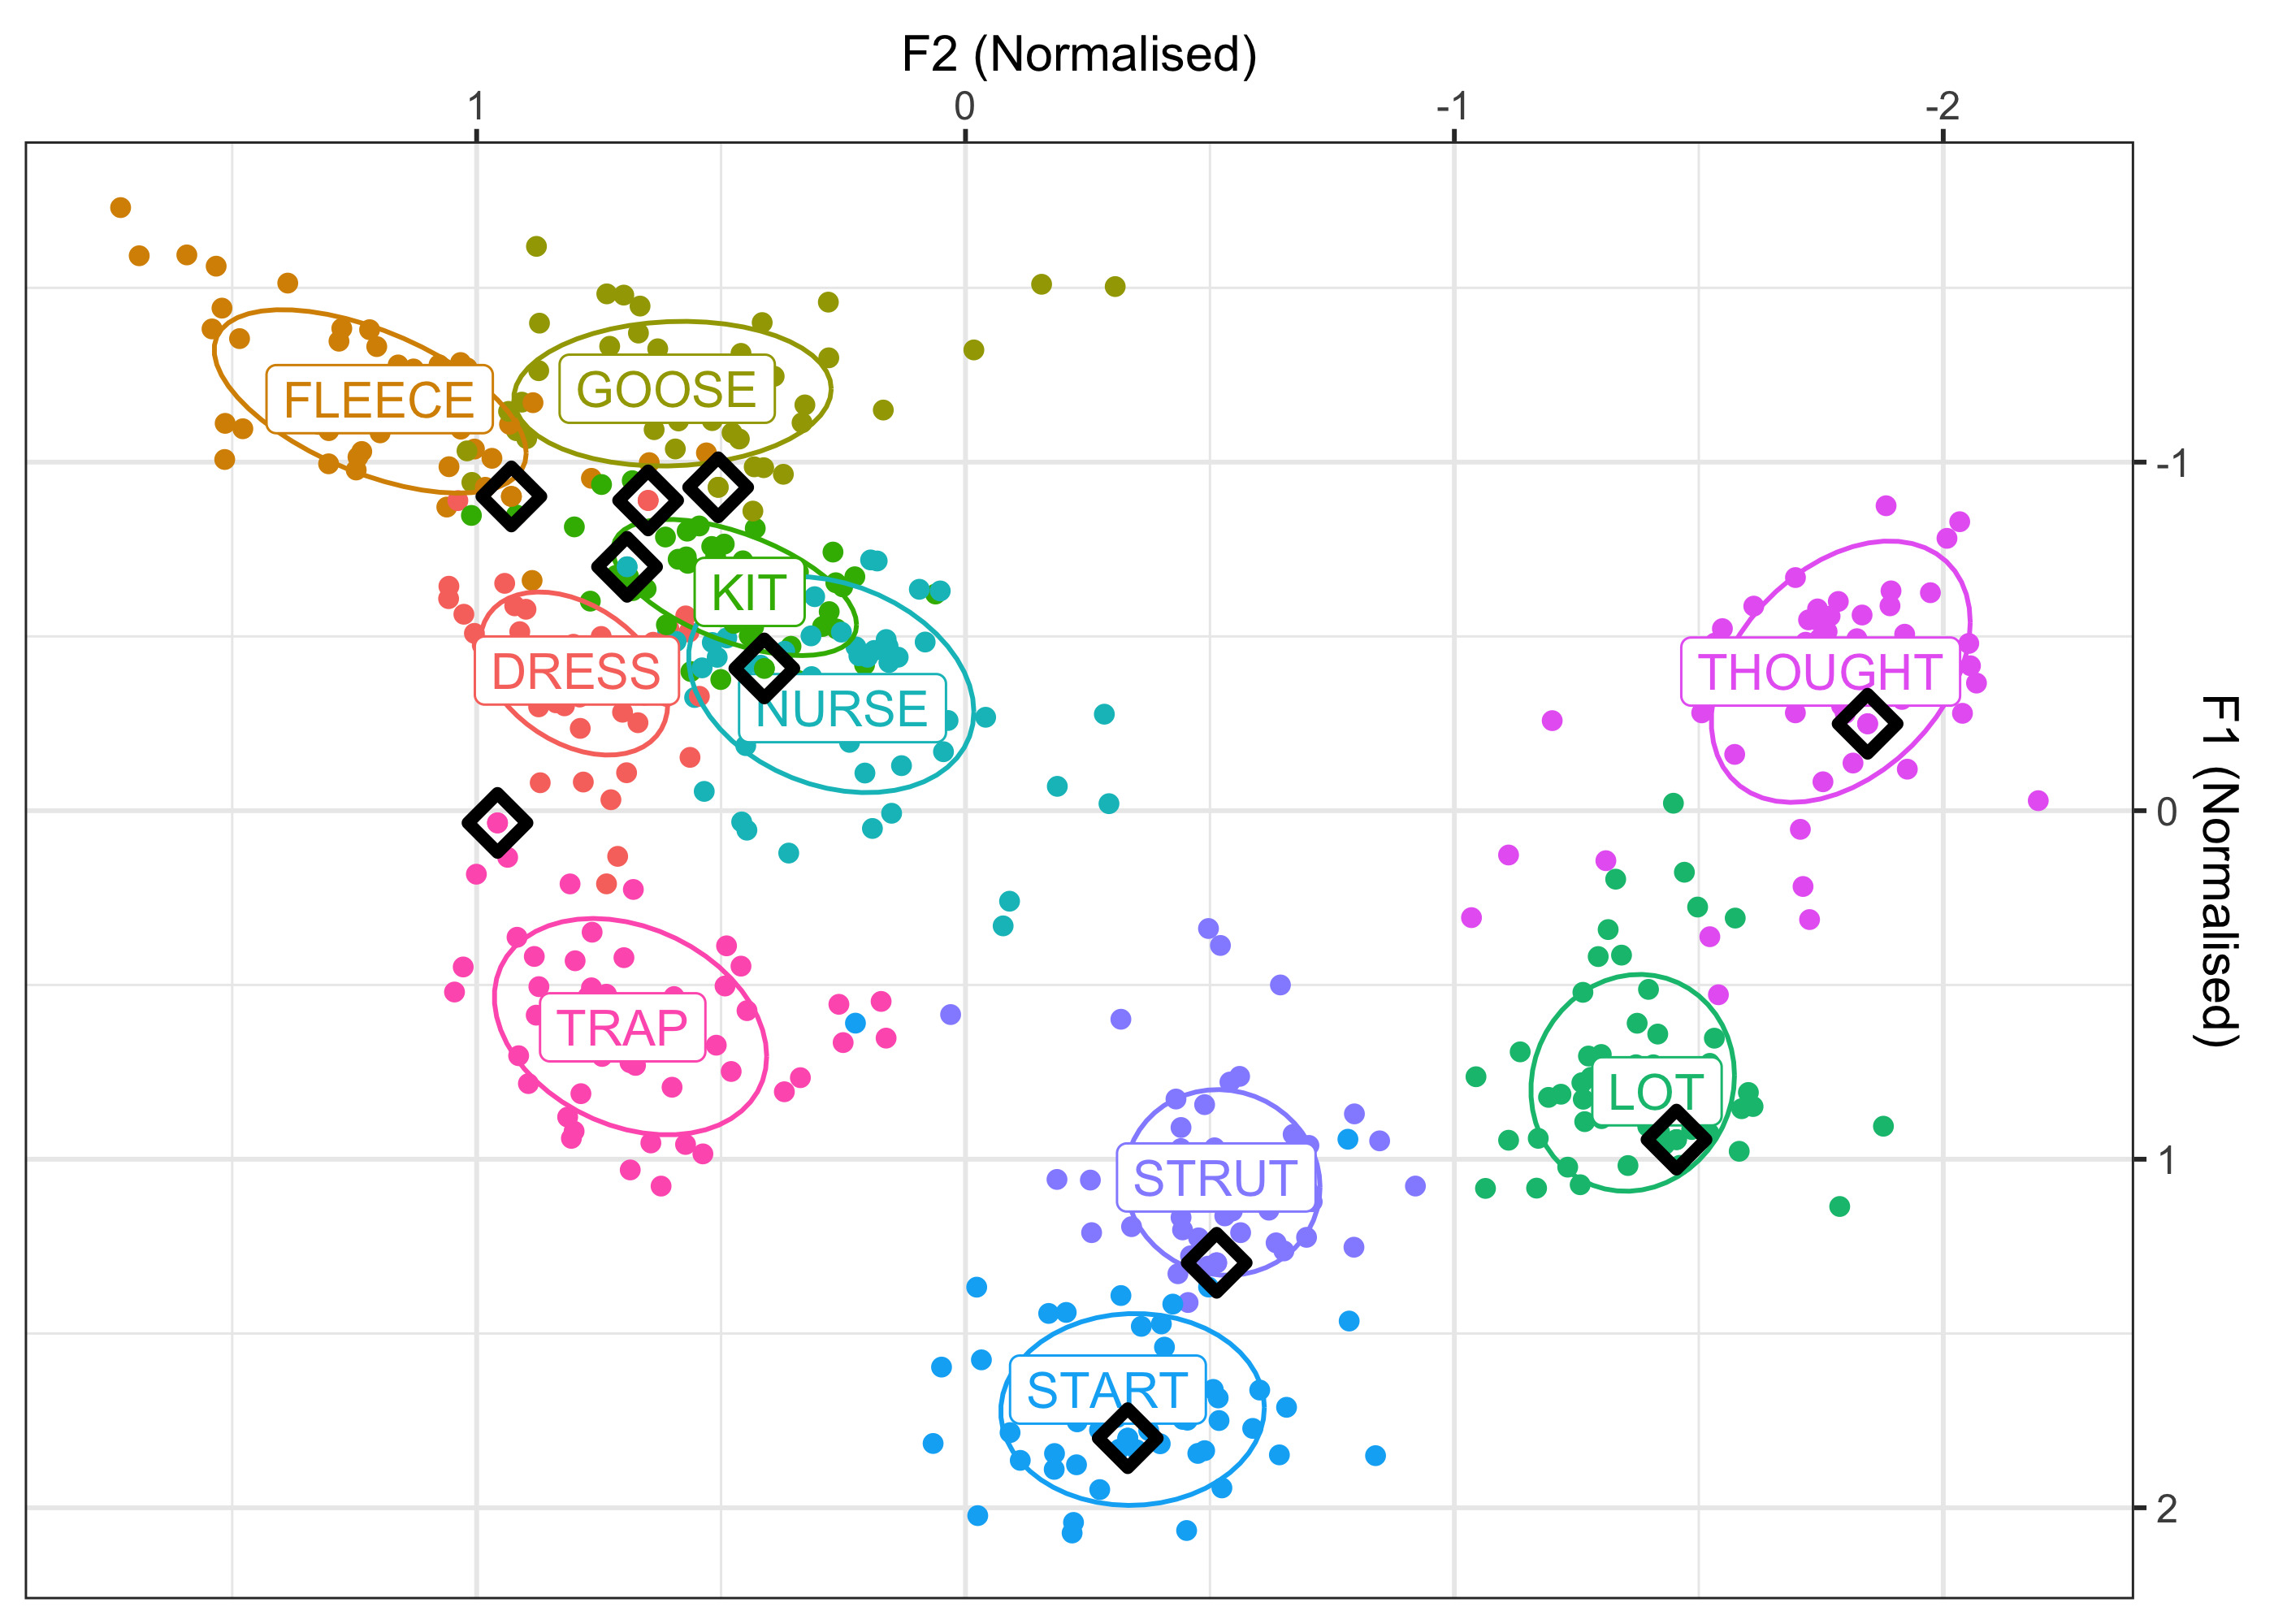
\includegraphics[width=\textwidth]{Figures/examplespeaker2.png}
\caption{Example vowel plot, showing mean positions of vowels for various speakers (coloured points), and for one particular speaker (black points). Ellipses show the variation within the population for each of the vowels.}
\label{fig:speaker_example}
\end{figure}

In the vowel plot, the mean formant values for one particular speaker are presented by the black points.  This speaker, relative to the population, has a front \textsc{goose} vowel, whilst their  \textsc{dress} is also quite high.   These are both innovative variants in the context of the local sound changes in progress.  For these two vowels, at least, this speaker seems to be ahead in both changes that were in progress at the time. Is this a coincidence? Or might we see this configuration if we look across multiple speakers? This paper investigates the degree to which a given speaker’s location in a single vowel is predictive of their location for other vowels, relative to the population.   If a speaker produces a front \textsc{goose} vowel that is innovative, for example, does this tell us anything about how they are likely to produce other vowels?  More generally, once we control for known sources of variation, such as anatomy and socio-demographic information, are speakers’ productions of each vowel independent of all other vowels?

This question is important both from the point of view of understanding vowel systems, and of understanding speakers.  Which (if any) sets of vowels tend to co-vary? and which (if any) sets of speakers tend to co-vary for which sets of vowels?  In terms of vowel systems – are there subsystems of vowels that appear to co-vary – potentially because they are structurally linked, or share socio-indexical associations?  Such questions cannot be answered by looking at vowels in isolation, but only at looking at the production of vowels as entire systems. In terms of speakers – the co-variation question gets to the heart of an ongoing debate in the sociolinguistics literature about the individual’s role in sound change – particularly with respect to identifying `leaders’ and `laggers’ of sound changes.  Is it coherent to identify people that are, in general, `leaders’ of sound change?  In other words, ``if one is a leader of sound change, does that mean that this person is advanced in all sound changes?" \citep{guy2016linguistic}.  Before we can even start to address questions such as the above, we need to develop methodologies that allow us to study co-variation.  That is the major goal of this paper.  We report on our methodology, and on an analysis which studies co-variation in NZE using that methodology.

In section \ref{sec:socio} we discuss the literature from sociolinguistics that leads us to predict patterns of co-variation across speakers, and in section \ref{sec:phon} we outline the factors from phonology that might lead certain vowels to operate as subsystems.   Our particular research questions are laid out in full in section \ref{sec:researchquestions}.

\label{sec:background}
\section{Background}
\subsection{Sociolinguistic co-variation}\label{sec:socio}
\subsubsection{Social meaning and sound change}
The sociolinguistic literature predicts that speakers might show non-independent realisations of sets of vowels, if the realisations carry some shared social meaning.
Social meaning is the indexical association between linguistic material, and some aspect of the “speaker as a social actor in the speech situation” \citep{eckertlabov2017}.   Aspects which are often used in sociolinguistic studies are associations with broad social categories such as class, age and gender --  macro-categories  which can often crudely reflect divisions of social interactions and experiences.  In producing a vowel, a speaker conveys not only a linguistic category, but also a range of social information about themselves (cf., e.g. \citealt{campbell2010sociolinguistic, eckert2018meaning}).

In the language change literature, social meaning is often assumed to accrue to individual variables (e.g. studies might be of the vowel \textsc{nurse}, or of medial /t/).   The study of phonetic variation and change has been built on a large number of increasingly sophisticated analyses of how specific isolated linguistic variables are used across different speakers and contexts, and how they change over time.   The vast majority of studies in this literature report on variation or change in an individual variable. From this, we have learned that the phonetic implementation of phonological variables can change radically across generations \citep{labov2001principles, trudgill1974social}, across contexts \citep{love2013football, foulkes201513}, and across social groups \citep{eckert2000language, mendoza2014homegirls, dickson2017class}. Even when multiple variables are investigated in the same study, they are nearly always examined in isolation of each other, with the exception of a few specific sound changes, which are hypothesised to be causally related (e.g. chain-shifts, see \citealt{gordon2002investigating, maclagan2007getting, hay2015tracking} and section \ref{sec:phon}).

By contrast, social meaning in the context of work on style and stance is interpreted as an indexical association between an aspect of the speaker and the full constellation of variants produced in context. \cite{eckert2019} states that “Sociolinguistic variables do not occur independently, but as components of styles.”   In contrast to the literature on language change, work on speaker style (e.g. ~\citealt{eckert2016variation, eckert2018meaning}), has focused more explicitly on individual speakers, exploring how linguistic styles, as collections of different phonetic variants, unfold over the course of a conversation. This literature argues that speakers display stylistic variation through combinations of variants, and the meaning of a particular variant cannot be properly interpreted in isolation of the landscape of other variables with which it co-occurs. Such analysis sheds light on how sounds are used in actual conversation, but the focus is usually on micro-level variation, often within a single speaker (e.g.~\citealt{becker2014linguistic,podesva2007phonation}).

Certain variants of different variables may share overlapping social meaning (for example `nerd', `diva', `country-oriented' or `laid-back' (see, e.g. \citealt{bucholtz2010white, podesva2008three, podesva2015country, podesva2011california}), leading them to be statistically associated in the types of speakers who produce them.  Or it may be that stylistic meaning is distributed – to be found in the combination of realisations of high variants of certain vowels together with front versions of other vowels.  Either one of these would lead to non-random co-variation between variants of different vowels, across speakers.  
In sum, the recent sociolinguistic literature and associated understanding of nuances of social meaning lead to clear predictions that stylistic variants may co-vary, and that sound changes will not operate independently of each other.

\subsubsection{Identifying Leaders and laggers}

An open question is whether the advanced variants of sound changes inevitably have shared social associations and thus tend to be used by the same speakers.  That is, if we found, in figure \ref{fig:speaker_example},  that there were patterns of co-variation across speakers, would it also be the case that for vowels undergoing change, speakers were uniformly advanced or conservative in their realisations of those vowels?

A growing literature dealing with potential co-variation amongst variables focuses on leaders in sound change. \cite{guy2016linguistic} asks: ``Are there socially identifiable leaders of change who tend to use all the innovative variants together, or are different innovations subject to differentiated social interpretations and individuated patterns of usage?'' (p.4). \cite{guy2013cognitive} identifies ``a dearth of research in the field that addresses whether clustering of variables actually occurs in the behavior of individuals'' (p.64).  He investigates pairwise correlations between 4 variables, and finds their relationships to be `weak'.  Since then, there has been a small flurry of studies investigating the question of whether variants of different variables cluster within speakers.

Studies include \cite{oushiro2016social}, who finds that a selection of structurally related and structurally non-related variables co-vary, based on São Paulo Brazilian Portuguese. \cite{watt2000phonetic} notes parallel changes in the \textsc{face} and \textsc{goat} vowels of Tyneside English, which seem to be distributed in a similar way across speaker groups, attributing the co-variation between the two vowels to a shared social meaning. This argument is also used by \cite{tamminga2019interspeaker}, who conducted a series of pairwise correlations across vowels undergoing change in Philadelphia, and finds correlations between three out of six investigated changes.  She addresses some of the methodological challenges, by working with a homogeneous group of speakers, in addition to statistically controlling for a number of social and linguistic factors. She argues that the co-varying vowel changes share some social meaning that is not shared by the others. \cite{becker2016linking} makes a similar claim, finding evidence for co-variation between the lowering of the \textsc{thought} vowel and a decrease in non-rhoticity for speakers from New York.  Becker proposes that young New Yorkers are trying to avoid association with a `classic New Yorker' persona (p.\ 97).  
The degree of co-variation may also depend on the type of variable.

\cite{waters2017one} report no correlations between leaders of one variable and leaders of any other based on pairwise correlations of five spoken morphosyntactic variables. In another study of morphosyntactic changes in writing, over a longer time period, \cite{nevalainen} find that some individuals were innovative on a collection of variables. They note, however, that no-one was progressive on all changes underway and that ``even among those predominantly progressive, the common pattern included not only in-between use but also conservatism with regard to some changes'' (p.\ 33).  In sum, the emerging picture appears to be that (when considered in a pair-wise fashion) some correlations can often be found, but that it is not the case that speakers tend to be uniformly `leaders' or `laggers' for all changes (see \citealt{tamminga2019interspeaker} for review). In other words, studies tend to find pairwise correlations between some, but not all, variables undergoing change.  

This is a topic of lively debate within sociolinguistics, but two methodological issues are pervasive.   First, when variables are changing over time and are systematically distributed across groups, there exists variation based on demographic information (such as year of birth), which needs to be controlled for in order for true individual effects to robustly emerge. Researchers who acknowledge this problem deal with it by looking for co-variation within a highly restricted sub-set of speakers who are socially more homogeneous (e.g.\ \cite{tamminga2019interspeaker}).  And secondly, the predominant statistical approach is to search for pairwise correlations between particular pairs of variables.  While potentially locally revealing, it does not reveal any broader systematic structure that might extend beyond particular variable pairs.  Thus, in order to build a system-wide account of co-variation, an improved methodology is required.

In sum, despite the preponderance of single-variable analyses, there are many reasons from sociolinguistics to expect that we might find sub-systems of variables which pattern together.   It is therefore crucial to develop methodologies to investigate patterns of co-variation across linguistic variables at scale, so that we can move towards a fuller understanding of the range of factors that influence and constrain language variation and change.

\subsection{Potential structural co-variation}\label{sec:phon}
Separately from considerations of social meaning and indexicality, there are phonological phenomena which may lead to predictions that certain vowels would pattern together across speakers. Any observed co-variation needs to be interpreted in the context of these potentially relevant structural phenomena.  We use the term `structural relationship' to refer to any type of co-variation that is driven by factors relating to phonological factors (such as changes in shared phonological features), contrast maintenance (such as chain-shifting), or system-wide evolutionary pressure (such as a drive toward symmetry).  Broadly construed, we use this term as a cover term for potential co-variation that is driven by forces that govern the structure of sound systems.

It is well understood that there are long-term evolutionary pressures on sound systems, and perhaps particularly on vowels.  Sound systems exhibit properties consistent with pressures towards symmetrical vowel spaces \citep{boersma1998functional} and vowel spaces that maximise dispersion and contrast \citep{martinet1952function, moulton1962dialect, liljencrants1972numerical, schwartz1997major}. \citet{soskuthy15} argues that such pressures interact to define stable states that determine the evolution of sound systems as wholes, as opposed to individual sound categories. Therefore, to the degree that such factors are indeed driving ongoing changes, and to which {\em individual speakers} may vary in the degree to which they are influenced by such pressures, we might expect to see co-variation between subsets of sounds that are, for example, jointly moving in a direction that increases overall symmetry.

\cite{fruehwald2013phonological,fruehwald2017role} proposes that co-variation can also arise through the shifting phonetic implementation of an entire phonological class, possibly defined in terms of phonological features.   A proto-typical case of this phonologically-driven parallel shift is the case of back vowels, which have been found, across dialects, to undergo fronting.   In such cases, \cite{fruehwald2013phonological,fruehwald2017role} suggests that speakers are shifting in their implementation of the feature `back', which affects multiple vowels in parallel.\footnote{An anonymous reviewer points out that the observed effects might also come about through a similar force acting independently within each vowel category, such as each vowel shifting forward to maintain contrast with its backer pre-/l/ allophone.}   A related consonantal example is presented in \cite{chodroff2017structure} who look at the Voice Onset Time (VOT) of English aspirated stops, finding correlations between VOT of the different stops, across speakers.  They argue that ``aspirated stops can be straightforwardly accounted for with a constraint that requires the talker-specific realisation of a phonetic property (e.g., glottal spreading) to be uniform across speech sounds. The uniformity constraint, which could extend to many other phonetic properties and sound classes, allows talkers to differ but imposes a common relational structure or pattern on their phonetic systems'' (p.\ 31).  The idea that there are phonetic uniformity pressures in language is previously argued for in \cite{keating2003phonetic}. 

Vowel chain-shifts are also a case where one might expect to find co-variation - cases of systematic relationships between adjacent vowels.  Some such relationships have been described as a `push' relationship, in which a vowel seems to encroach on another's space, leading to a potential retreating movement by the encroached-upon vowel, and others as a `pull' relationship, in which a vowel's movement leaves a vacuum, into which another vowel may move \citep{gordon2002investigating, lubowicz2011chain}. In NZE, the short front vowels have been argued to be in a chain-shifting relationship, with \textsc{trap} and \textsc{dress} raising and \textsc{kit} centralising. \cite{hay2015tracking} have argued that the lexical frequency effects observed in the changes support a chain-shifting interpretation, in which the system evolves away from configurations leading to perceptual ambiguity. 

Some attempts to demonstrate causality in chain-shifts have employed the same methodology used to look for leaders in sound-change – pairwise correlations, at the individual level, between productions of associated vowels (e.g. \citealt{gordon2004new, boberg2019closer, kendall2017regional}). Such correlations can provide excellent evidence that chain-shifting not only exists, but is a phenomenon that can actually be observed within individual speakers - speakers who are advanced in one vowel in the chain may be more likely to be advanced in all - their advanced variants in one category having potentially `pushed' on their variants in an adjacent category. It would, after all, be possible that chain-shifts don't unfold in this manner - but rather exist at the population level, with different sets of speakers pushing forward the changes within the different vowels. Do chain-shifts lead to co-variation at the level of the individual?

Looking at co-variation within individuals, \cite{gordon2004new} show for speakers of NZE that the degree of innovation in \textsc{trap} (auditorily assessed) was statistically correlated with the degree of innovation in \textsc{dress}, whilst \textsc{dress}-raising was also correlated with \textsc{kit}-centralisation. Although this may suggest that the chain-shifting relationship exists at the level of the individual, their analysis does not completely rule out the possibility that the correlations arise because the sound changes are unfolding over the same time period.  As speaker year of birth is not controlled for in the correlation analysis, we can not draw strong conclusions.

\cite{soskuthy2017closing}'s, in an analysis of changes in NZE diphthongs, attempt to control for year of birth and known effects from social variables.  They fit a mixed-effects regression model to the diphthongs, extracting the speakers' random intercepts, which is used as an index of how advanced they are in the change beyond the model's fixed effects. The results revealed that the intercepts from the \textsc{price} and \textsc{face} models were significantly correlated, suggesting that this relationship was causal - given that the effects of year of birth and known social factors were controlled for in the modelling step.

Chain-shifting, then, is one area where researchers have explicitly attempted to look for structural relationships between vowel positions across speakers.  However, the focus has not been on a system-wide analysis, but rather on pair-wise correlations between neighbouring vowels.   A system-wide methodology which controls for potential confounds is required to (a) verify whether chain-shifts do exist at the level of the individual (as opposed to being sets of interlinked changes which unfold at the population level), and (b) avoid falsely attributing co-variation which could be due to structural chain-shifts to social factors, as outlined above.

In sum, a variety of structural factors predict that over a reasonable time-span, we might expect to see some vowels moving in ways that are dependent on each other. Whether these forces are operative at the level of the individual is unclear, but it is certainly a possibility.  These factors therefore need to be taken into consideration when investigating the question of whether there are `leaders' and `laggers' in sound change.  The very best evidence for this would come from co-varying vowels for which there is no obvious structural link.

\subsection{Interim Summary}
Despite the fact that the study of language variation and change has focused largely on the isolated variable, there are a number of phenomena in the literature that might lead us to expect some co-variation across linguistic variables.  We note that these are not at all mutually exclusive, and, indeed, it is possible (or perhaps even likely) that all of the above phenomena play a role in the evolution of sound systems.   For this reason it is important to move beyond pairwise comparisons between variables hypothesised to be linked, and look simultaneously at the implementation of a range of sounds to gain a holistic view of patterns of co-variation across them.

\section{Research questions}
\label{sec:researchquestions}

As outlined above, there are many questions, both in sociolinguistics and phonology, which require methodologies for the study of co-variation across the entire vowel space.   Developing such a methodology is our primary goal.\\
{\bf Primary Goal of Project}: To develop a methodology that enables the analysis of systematic co-variation.   Our data-set is a large set of recordings capturing the history of NZE.  The successful deployment of the methodology allows us to directly address several questions identified in the literature above, in the context of NZE,  namely:  \\
{\bf Research Question 1}:  In NZE, can we identify individuals who generally `lead' or `lag' in sound change, in a way that can be observed across multiple ongoing changes?\\
{\bf Research Question 2}:  Are identified patterns of co-variation explainable by structural factors (particularly - the short front vowel shift), or not?  If we exclusively find co-variation associated with the chain-shifting vowels, for example, we can conclude that the vowel shift is manifest at the level of the individual, but cannot conclude that we have evidence of associations potentially driven by social meaning.  However if we (also) find co-variation amongst vowels for which there is no clear structural explanation, such co-variation may be driven by social meaning, as predicted by the sociolinguistic literature.   We note that our methodology allows us to identify candidates for socially-driven co-variation, but not to find definitive evidence for them, which would require a careful analysis of the social meaning itself, within the identified candidate clusters.   Such an approach is outside the scope of this paper.   

Our primary aim is to develop a robust methodology which, for the first time, allows system-wide patterns of co-variation to be identified.



\section{Methodology}\label{sec:methodology}

This section outlines the methodology in detail, providing a general overview of the approach, then detailing the data-set, and the steps involved in data processing, normalisation, fitting the models, and conducting the principal components analysis.
Following guidance in \cite{roettger2019emergent}, all data and code are provided in the \hyperref[sec:supplementarymaterials]{Supplementary Materials} or accessible directly at \url{https://nzilbb.github.io/Covariation_monophthongs_NZE}. All code was written in R version 3.6.3 \citep{R2018}.


\subsection{Summary of methodological approach}

%Analysing the monophthongs of NZE, we aim to develope a methodology that can identify sub-systems within the vowel space -- pairs or sets of vowels that are interconnected, when well-known sources of co-variation (anatomical, year of birth) are controlled. We are particularly interested in the degree to which any patterns of co-variation might relate to patterns of ongoing sound change. Most of the NZE vowels have changed substantially over the 118 years of recordings we analyse.  We ask whether there are any persistent systematic linkages between the realisations of these vowels.  When we control for a speaker's year of birth and gender, does the realisation of one monophthong predict the realisation of others, or are all the changes spreading independently through the population?  

Our data covers 118 years of time, during which NZE, a relatively new variety of English, was being formed.  The speakers with the earliest years of birth, of course, have vowel spaces that resemble each others' more than they resemble the vowel spaces of speakers born several generations later.  If we simply take a large number of speakers and look at whether the realisation of one vowel is predictive of the realisation of a second, we would find many significant patterns of `co-variation' across vowels that are statistically linked simply due to the fact that they have both undergone substantial change during the same period. This is inevitable given the time-depth of our data. Such correlations would not necessarily reveal any systematic link between the sounds, apart from the fact that they happen to be changing simultaneously. This, of course, can be meaningful in and of itself, but it is difficult to establish causal links across such time series. Thus, this type of cross-speaker correlation is not the focus of this paper.  We also know, from past work, that many changes will show gender effects \cite{gordon2004new}. So at any given point, we are likely to find that female speakers' vowel spaces look somewhat different from male speakers.
However what we are interested in is whether the realisations of two vowels are systematically related within speakers, over and above the fact that the sound changes happen to have unfolded over the same time period and be led by certain groups of speakers. 

Our methodology attempts to remove these sources of co-variation by controlling for year of birth and gender in our statistical models.  Holding constant year of birth and gender, can we still see relationships between vowels, such that, at any given time, speakers who are advanced in one vowel change are also likely to be advanced (or perhaps conservative) in one or more other vowel changes?  That is, can we find systematic co-variation that is not caused simply by the fact that two vowels are moving over the same time period and being led by the same broad group of speakers, but rather, that can be isolated as being systematically linked within individual speakers?

In order to address our research questions, we introduce a novel analysis procedure that aims to overcome the long-standing difficulties with the study of phonetic co-variation, and apply it to a corpus of NZE that has a large number of speakers and considerable time-depth. The core steps are:

\begin{enumerate}
    \item Compute estimates of how  speakers differ from the rest of the population in terms of their realisations of different vowels (based on their F1 and F2 values). This step involves statistically modelling formant frequencies and controlling for various predictors of change in the data. From these models we can extract intercepts for each speaker, which are used as a measure of how they differ from the rest of the population for each vowel (see \citealt{drager2012exploiting}, \citealt{fruehwald2013phonological}).
    
    \item Run a Principal Component Analysis (PCA) on the resulting data set of speaker intercepts. This will allow us to identify whether any patterns exist in terms of speakers being advanced in groups of vocalic variables, i.e.\ is there evidence of certain vowels co-varying together in a theoretically meaningful way.
    
    \item Once the resulting Principal Components (PCs) have been interpreted, we need to confirm that there is no statistical relationship between the speakers who drive the components and any of the variables used in the initial modelling procedure, i.e.\ are the PCs driven by known sources of co-variation, such as year of birth, or are they instead representative of co-variation that exists independently of those sources?
    
    % that speakers who co-vary within the PCs do so independently of known predictors of change.

\end{enumerate}

% Our data set is comprised of monophthongs from the Origins of New Zealand English corpus (ONZE)~\cite{gordon2007onze, gordon2004new}). We make use of the fact that the ONZE corpus has an extensive number of tokens available for analysis, from speakers born over several generations. This provides an ideal resource for testing whether there is co-variation of phonetic variants across different speakers. In addition, ONZE's substantial time depth and well documented evidence of sound change will allow us to identify whether there are speakers who lead along the changes represented by these phonetic variants. Building on work in~\cite{soskuthy2017closing}, we fit separate mixed effects regression models to each vowel category in the data set. As we explain further below, the models include year of birth as one of the predictors, and so are able to shed light on co-variation among variants while controlling for diachronic changes.

% To do this, we extract by-speaker random intercepts (a measure of whether the speaker's formants are higher or lower than we would expect, given their year of birth and gender), then analyse these intercepts using Principal Component Analysis (PCA). This method provides a way to expose the correlation structure of different phonetic variants across speakers, allowing us to identify whether certain subsets of variables tend to cluster together in their usage.



\subsection{Corpus}
\label{sec:methods_corpus}

The data analysed in this paper come from the ONZE corpus \citep{gordon2007onze}, which comprises three sub-corpora: the Mobile Unit recordings (MU), the Intermediate Archive (IA), and the Canterbury Corpus (CC). We have combined this with the Canterbury Regional Survey \citep{darcy2017discourse}. The ONZE corpus is unique in that it provides the longest record of transcribed NZE in existence, with speakers born over a 137 year time period (1851-1988). The speech samples were collected during interviews, with much of the speech being spontaneous. The combined corpora contain over 600 different speakers, who come from a range of social backgrounds and geographical locations, predominantly from within the South Island of New Zealand. 

\subsection{Data processing}
\label{sec:methods_processing}

The corpora are searchable through the LaBB-CAT database \citep{fromont2008onze}, where large volumes of speech have been force-aligned at the phoneme level using the HTK-Toolkit \citep{young2002htk}. We initially extracted all vowel tokens that contained any of the 12 monophthongs of NZE (\textsc{dress, fleece, foot, goose, kit, lot, nurse, start, strut, thought, trap}, comm\textsc{a}), querying all 636 available speakers. We then automatically extracted F1 and F2 values at the midpoint of each vowel token using Praat \citep{praat2018}, resulting in a data set of over two million vowel tokens. In order to ensure sufficient quantity and quality from this data set, we applied a number of filtering and data processing steps. These are summarised below and in Figure \ref{fig:data_filtering}, with a more detailed explanation included within the \hyperref[sec:supplementarymaterials]{Supplementary Materials} (including the code used at each step).

%%%%%%%
%data_filtering
%%%%%%%

\begin{figure}[!t]
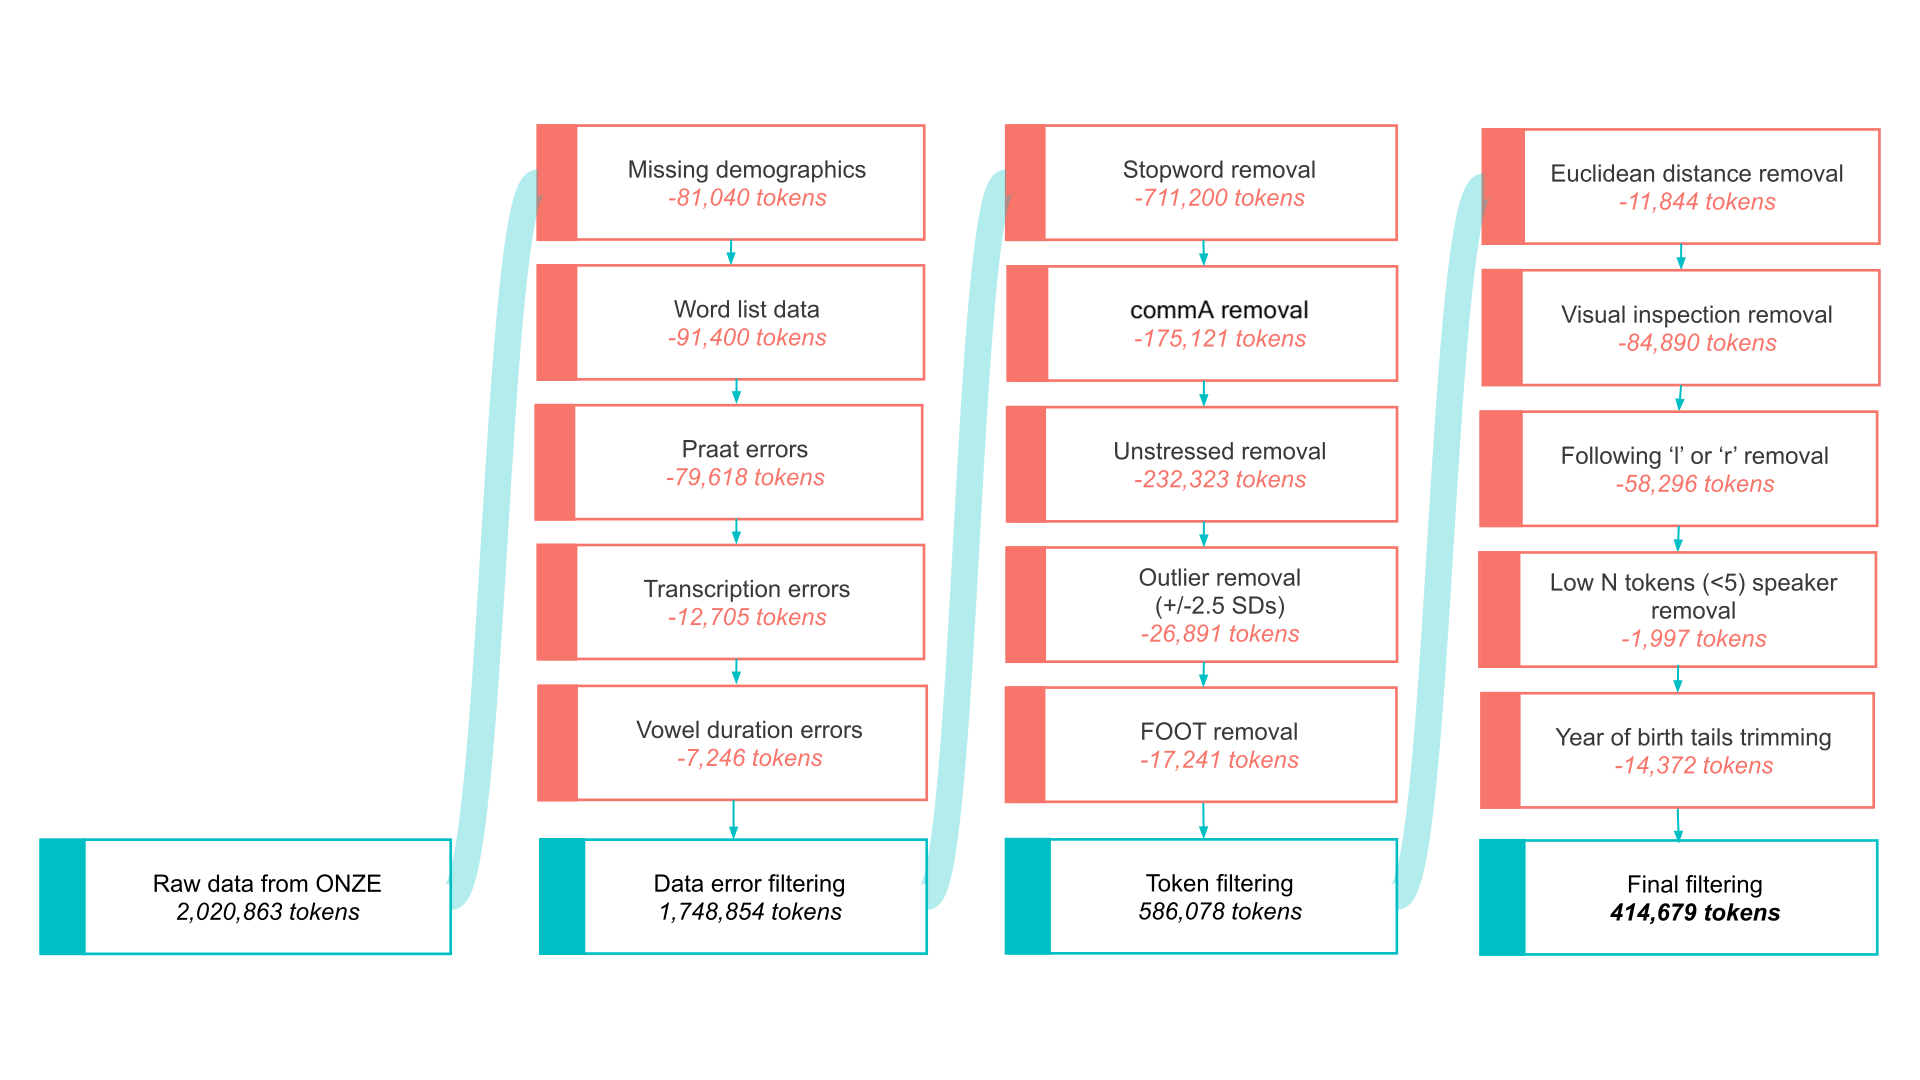
\includegraphics[width=\textwidth]{Figures/Data_filtering.png}
\caption{Steps taken to obtain the final data set used in the subsequent analyses}
\label{fig:data_filtering}
\end{figure}

%%%%%%%

Firstly, we removed any speaker whose birth year or gender was unknown to us.  We then removed any data that came from a word list reading style, or where Praat was unable to extract an F1/F2 measurement. As the data was force-aligned, we also ensured that all tokens had an F1 under 1000Hz, had a valid orthographic and phonological transcription and a vowel duration between 0.01 and 3.0 seconds. Next, we removed all tokens that occurred in a list of 82 stopwords (high frequency grammatical words, see the \hyperref[sec:supplementarymaterials]{Supplementary Materials} for the full list) as these words are prone to phonetic reduction (see \citealt{hay2015tracking}). We also removed all unstressed tokens in the data set (including all tokens coded as comm\textsc{a} and tokens without any lexical stress coding in CELEX \citep{baayen1995celex}. In order to remove outliers, we filtered out all tokens that had an F1 or F2 value that was $+/-$2.5 standard deviations from the mean formant value per speaker, per vowel. Upon inspecting the token counts for each speaker, we observed relatively low counts for \textsc{foot}. As the statistical modelling approach we use requires that all speakers should have sufficiently high token counts across all vowels, we decided to remove all \textsc{foot} tokens.

In order to further ensure that our data set contained reliable F1/F2 measurements, we implemented three additional filtering steps which were applied on a speaker-by-speaker basis (rather than token-by-token). Firstly, we implemented a minimal vowel-space dispersion requirement.  If, for some reason, automatic formant tracking failed for most tokens for a single speaker, the vowel-based outlier-removal processes (described above) would not necessarily remove the mis-measured tokens.  If the distributions of all vowel categories overlap each other, then no individual token is going to be flagged as an outlier for any specific vowel category.  

In order to identify speakers with vowel spaces that do not contain distinguishable categories, we calculated the mean Euclidean distance between all of the vowel categories produced by a speaker.  This was done to obtain a measurement of dispersal for each speaker.  We identified 14 speakers who had particularly small values for this measurement (those that were smaller than the population's mean Euclidean distance by $-2$ standard deviation), which indicated that there was little variation in the location of the formant measurements across all the vowels, i.e.\ their vowel realisations overlapped across lexical sets. As a consequence, these speakers were removed from the data set. This led us to our second speaker filtering step, which involved manually inspecting the vowel spaces and density distributions of the F1/F2 values for each of the remaining speakers. Following this, we decided to remove a further 76 speakers from the data set, for whom the distribution of the vowels was clearly atypical. Finally, 13 additional speakers were removed who had year of birth values at the tails of the distribution.  They were removed as we found that the distribution of speakers with the latest or earliest year of birth values was very sparse, and these speakers ended up exerting an unduly large influence on our statistical models (resulting in overfitting). Note that while exclusion of these speakers improves our models, it does not affect our main findings.

Next, we removed all tokens where the vowel was followed by /l/ (because NZE has some vowel mergers before /l/ \citep{thomas2005pleasant, bauer2007new}) or /r/ (because rhoticity has been variable over the history of NZE \citep{hay2005rhoticity}, and will affect vowel quality).  Finally, we removed any speaker with fewer than 5 tokens for any of the vowels. This was done in order to ensure every speaker had sufficient data for the analyses (token counts for each speaker can be found in the \hyperref[sec:supplementarymaterials]{Supplementary Materials}). The final data set comprises 414,679 tokens across 10 monophthongs, from 481 speakers (225 female, 256 male), born between 1864--1982. A summary of the token counts per vowel can be found in Table \ref{tab:token_counts}.

\begin{table}[t]
\caption{Number of tokens per vowel and their percentage in the final data set.}
\centering
\begin{tabular}{lcc}
\\
  \hline
  Vowel & N Tokens & \% \\ 
  \hline
  \textsc{nurse} & 16,891 & 4.1 \\ 
  \textsc{start} & 21,217 & 5.1 \\ 
  \textsc{goose} & 26,432 & 6.4 \\ 
  \textsc{thought} & 28,201 & 6.8 \\ 
  \textsc{trap} & 32,284 & 7.8 \\ 
  \textsc{lot} & 35,228 & 8.5 \\ 
  \textsc{fleece} & 49,757 & 12.0 \\ 
  \textsc{strut} & 50,907 & 12.3 \\ 
  \textsc{dress} & 69,925 & 16.9 \\ 
  \textsc{kit} & 83,837 & 20.2 \\ 
  \hline
  \textbf{Total} & \textbf{414,679} & \textbf{100} \\ 
  \hline
  
\label{tab:token_counts}
\end{tabular}
\end{table}

\subsection{Normalisation}
\label{sec:normalisation}

At the most basic level, it is well understood that the formant structure of vowels is systematically linked to anatomical features -- most notably the length of the vocal tract \citep{fant1970acoustic, stevens2000acoustic}. Vowel space size can also differ through a combination of anatomical factors and articulatory habits, such as degree of hyperarticulation \citep{lindblom1990explaining}.   A variety of normalisation techniques have been developed to try to remove this source of variation. In this paper, we adopt a modified version of the Lobanov normalisation procedure \citep{lobanov1971classification}, which is intended to ensure that the F1 and the F2 measurements for different speakers cover approximately the same space.  This should remove effects of vocal tract length and vowel space size. Note, however, that there may be effects related to anatomy \citep{johnson2018} and/or articulatory setting \citep{honikman1964articulatory} which affect some parts of the vowel space more than others \citep{johnson2018}.   If this is the case, then we might expect the vowels most affected by such variation to systematically co-vary across speakers. 

Moreover, the question of whether articulatory setting is a truly trivial source of variation is by no means straightforward.  Changes within the Californian Vowel System, for example, have been attributed to variation in jaw setting, which may be more typically associated with certain personas \citep{pratt2017jaw}.
Moreover, recent work on Glasgow English by \citet{soskuthyandstuartsmith20} shows that articulatory setting itself -- in their case, tongue body position as cued by F3 -- can be the subject of diachronic change, resulting in shifts in formant values that manifest across all sonorants. \citet{soskuthyandstuartsmith20} argue that the distinction between segmental and voice quality changes is necessarily fraught, insofar as they often operate on the very same articulatory features and acoustic cues. This can make it difficult to distinguish between parallel shifts across different sounds and changes in articulatory setting. We take a conservative approach in this paper by adopting a normalisation procedure that factors variation that is manifest across all formants, but acknowledge that such anatomical processes are potentially important in shaping vowel systems.

We normalised the formant frequencies using an adapted version of the Lobanov method \citep{lobanov1971classification}. Lobanov's formula normalises the formant frequencies on a speaker intrinsic basis and has been widely reported and used as the optimal method for normalisation \citep{adank2004comparison}. Yet, when we consider the data that we intend to normalise, a number of issues arise when applying the Lobanov method. The formula normalises each speaker's formant values by subtracting the raw formant value from the mean of all formant values; then dividing by the standard deviation of all formant values; see Equation \ref{eq:lobanov} (where $i$ is an index denoting a given speaker's formant (i.e. F1/F2); $\mu$ is the mean; and $\sigma$ is the standard deviation). This is convenient when the data set is balanced, i.e.\ each speaker has roughly equal token counts per vowel, as well as roughly equal token counts per speaker.

\begin{equation}
F_{lobanov_i} = \frac{(F_{raw_i}-\mu_{raw_i})}{\sigma_{raw_i}}
\label{eq:lobanov}
\end{equation}

 However, our data set contains spontaneous speech from hundreds of speakers, and as a consequence, has large variability in the token counts per vowel and per speaker. When using Lobanov's formula in this situation, the normalisation procedure is prone to bias towards vowels with larger token counts, and thus instability when different speakers produce different counts across vowels (e.g.\ in our data set \textsc{kit} is more common than \textsc{nurse}, so the calculation of $\mu$ and $\sigma$ will be weighted toward KIT and away from NURSE). To resolve this issue, we introduce a formula that is better suited to imbalanced data sets, which we will refer to as \textit{Lobanov 2.0}; see Equation \ref{eq:lobanov2.0}. In this adapted version, the primary difference is that means are calculated per vowel category, then a mean of means (i.e.\ the mean value calculated across the individual vowel means) is subtracted from the raw formant value. This value is then divided by the standard deviation of the mean of means, giving the normalised formant value.\footnote{See the \hyperref[sec:supplementarymaterials]{Supplementary Materials} for the implementation of this formula in R, with further discussion on the differences in normalised values produced by the two methods.}

\begin{equation}
F_{lobanov2.0_i} = \frac{(F_{raw_i}-\mu_{(\mu_{vowel_1},\cdots,\mu_{vowel_n})})}{\sigma_{(\mu_{vowel_1},\cdots,\mu_{vowel_n})}}
\label{eq:lobanov2.0}
\end{equation}


\subsection{Creating speaker intercepts}
\label{sec:intercepts}

In order to analyse co-variation in the data set, we must first extract a measure of how each speaker's realisations of the different vocalic variables compare with those of the other speakers. The goal is to assess how deviant each speaker is for each vowel, given where we would predict them to be for their year of birth and gender, and also controlling for variability in speech rate.  To obtain this measure, we exploit the random intercepts produced by mixed models, which provide estimates of speaker variability, whilst keeping other variables constant (see \citealt{drager2012exploiting}). This approach runs counter to traditional applications of mixed-effects modelling, where fixed-effects are the main focus of interest. Instead, it is the random effect of speaker in the models that we are interested in. The fixed-effects are included primarily as variables we wish to control for.

Take for example the vocalic variable of F1 for \textsc{dress}, which has previously been reported to have undergone sound change in NZE \citep{maclagan2007getting, gordon2007onze, hay2015tracking}. If we were interested in testing whether year of birth can predict changes in F1 \textsc{dress}, we could use a mixed model in which fixed effects of \textit{year of birth} and a random effect for \textit{speaker}, in which the fixed-effect is the variable of interest and the random effect is included to account for variation between speakers. Such a model may tell us that there is a significant effect for year of birth, and thus evidence for a sound change. If we inspect the random intercepts for the speaker variable, we can assess how advanced each speaker is in relation to other speakers with similar year of birth values.

Intercept values from mixed models are typically normally distributed\footnote{The intercepts from the modelling procedure described below are indeed normally distributed as shown in the Supplementary Materials.} as a continuous variable, with values centered around 0, making them comparable across different models. If we take the F1 \textsc{dress} model example, a positive speaker intercept indicates a deviation from other speakers born around the same time in a positive direction (which corresponds to an articulatorily lower vowel). On the other hand, a negative intercept indicates a deviation in a negative direction from other comparable speakers. In this case, this is also the direction of the sound change, as \textsc{dress} has undergone raising in NZE. Thus, a negative intercept would mean that our speaker is more advanced than others in terms of F1 \textsc{dress}. The further the intercept is from 0, the more the speaker deviates from the rest of the population. Thus, the speaker intercepts provide an estimate representing variability across speakers, but crucially keeping all other predictive variables constant. See Figure \ref{fig:F1_speaker_intercepts} for a visual demonstration of how these intercepts can identify speakers who are advanced in the NZE short front vowel shift.

%%%%%%%
%F1_speaker_intercepts
%%%%%%%

\begin{figure}[!t]
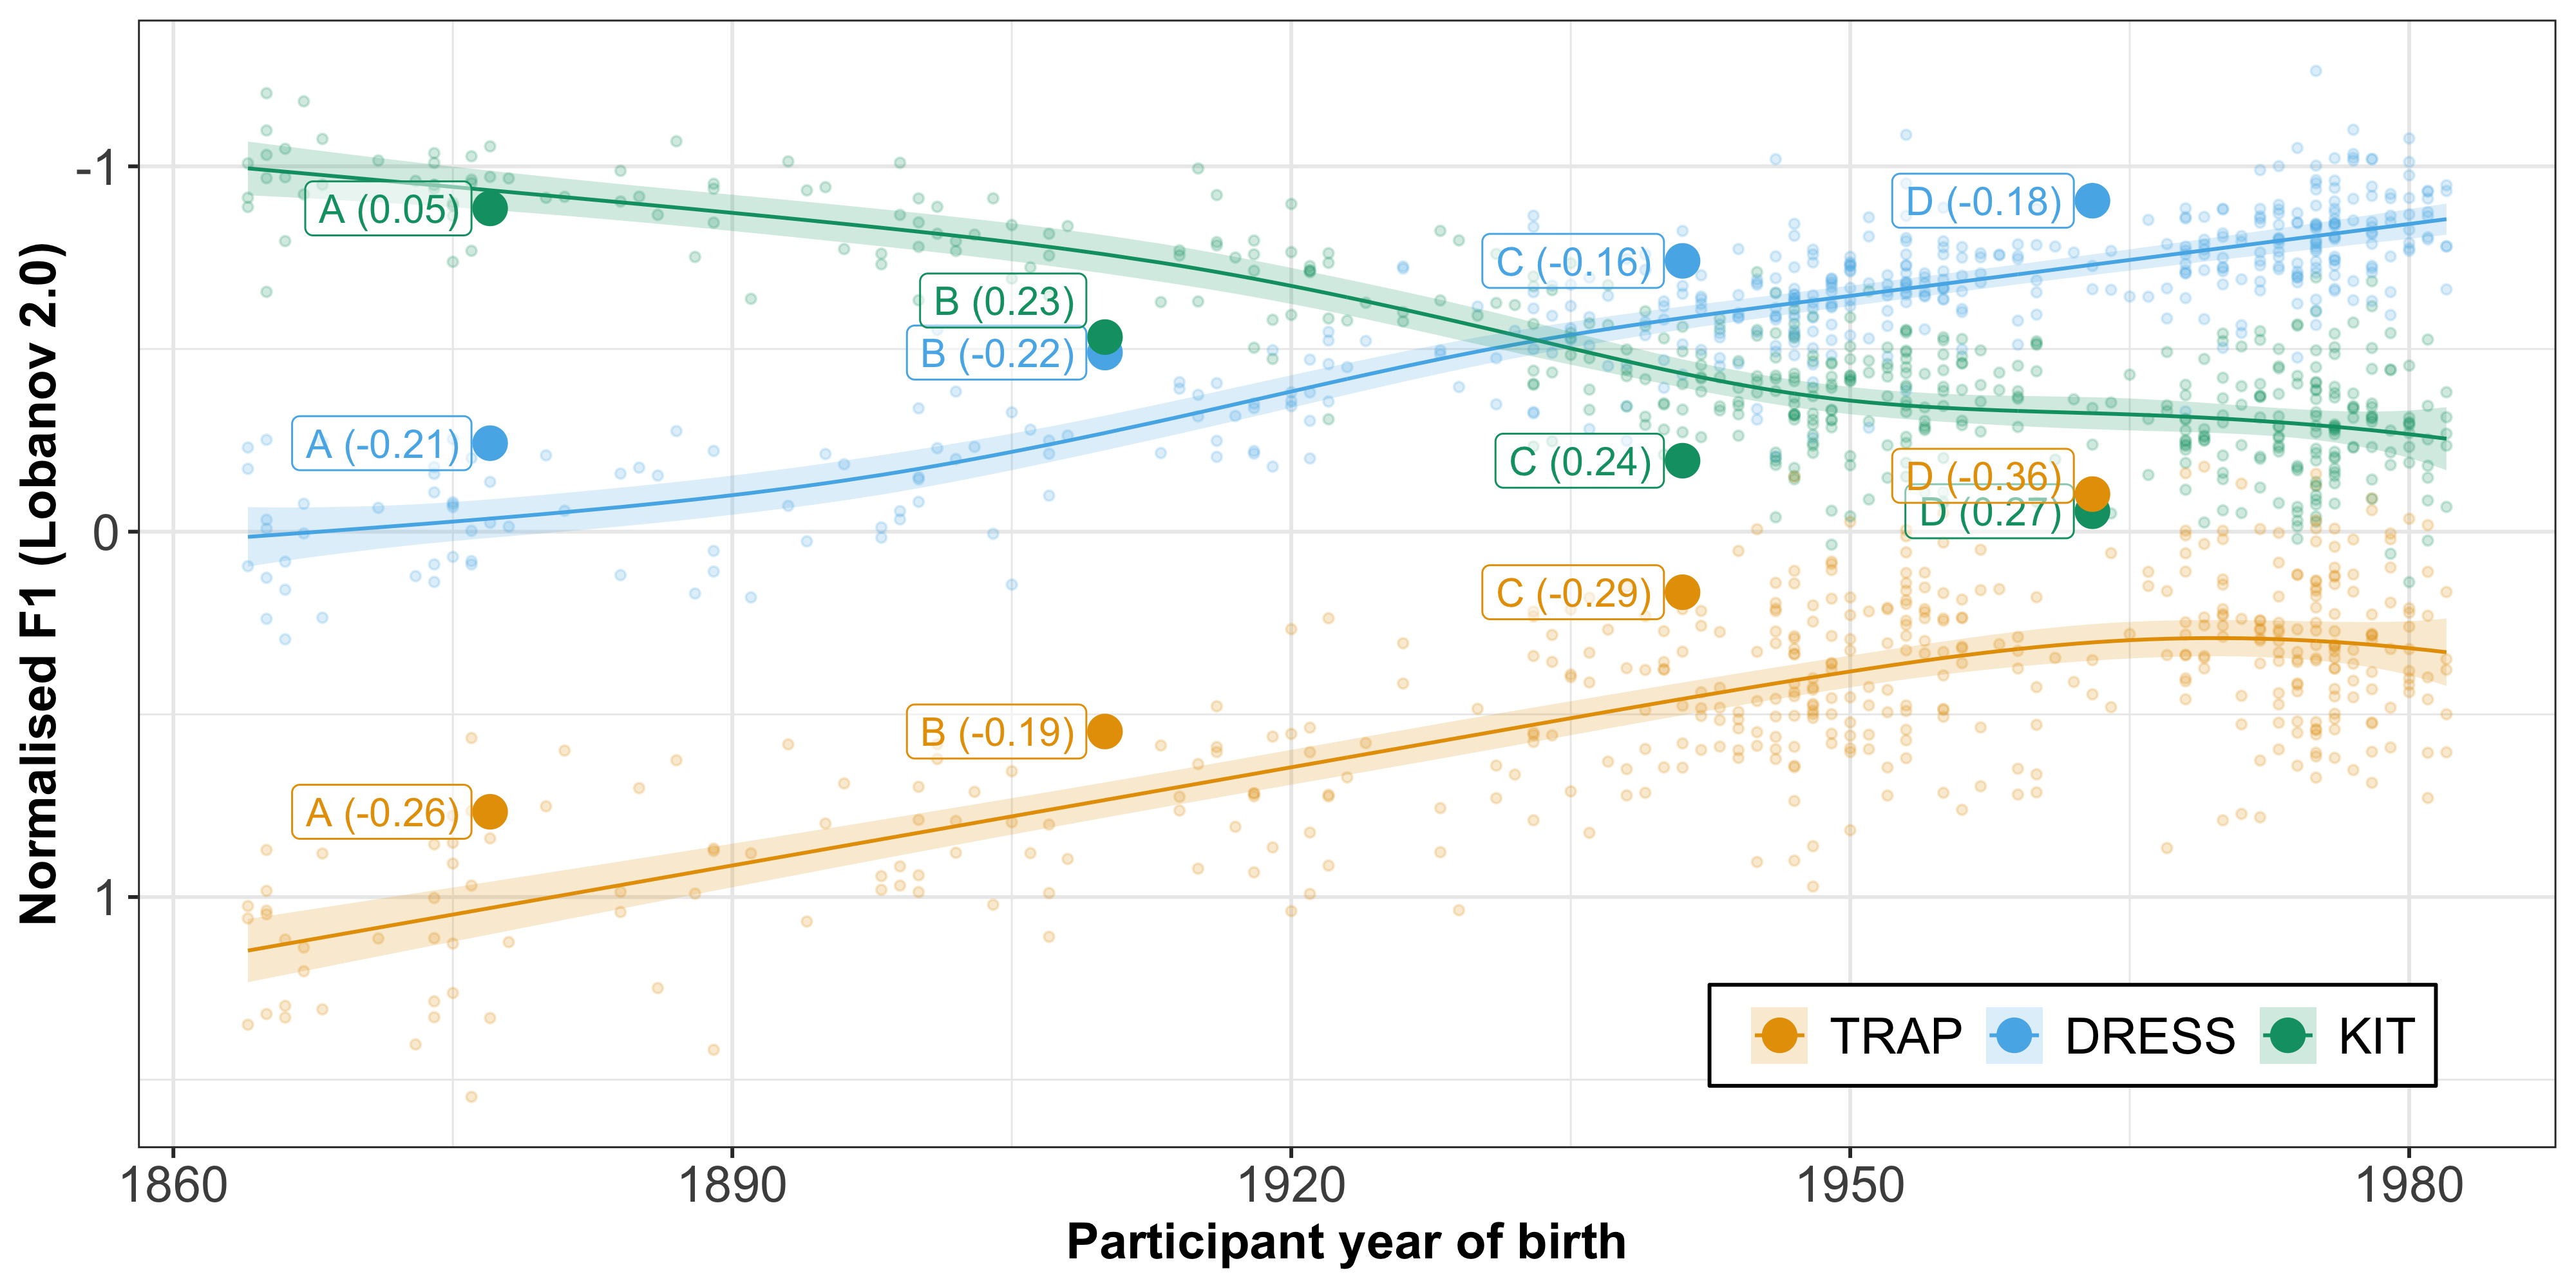
\includegraphics[width=\textwidth]{Figures/F1_speaker_intercepts.png}
\caption{Visualisation of change in F1 (normalised) for \textsc{trap, dress} and \textsc{kit} over the period of change in ONZE. GAMM smooths are added to show direction of change, whilst individual points represent each of the 481 speaker's mean F1 values for the three vowels. Four speakers (A, B, C and D) have been highlighted on the plot as they all have random intercepts (given in brackets) which indicate they are advanced in the direction of change (negative intercepts for \textsc{trap} and \textsc{dress} and positive for \textsc{kit}). Typically, the larger the distance from the smoothed line, the larger the absolute value of the intercept.}
\label{fig:F1_speaker_intercepts}
\end{figure}

%%%%%%%

Speaker intercepts from linear mixed effects regression models have been used to index speaker advancement in sound change \cite{drager2012exploiting, soskuthy2017closing}.   The data we analyse here contains some non-linear effects, and thus an appropriate modelling technique to obtain the speaker intercepts from our data is generalised additive mixed modelling (GAMMs).  This is because we want to model the normalised F1 and F2 of each of the 10 monophthongs separately, whilst also reliably capturing non-linear changes across time (see \citealt{winter2016analyze}, \citealt{soskuthy2017generalised}, \citealt{wieling17tutorial} and \citealt{chuangetal20} for introductory tutorials on GAMMs). We fitted separate models to normalised F1 and F2 for each of the 10 vowels in the data set, giving 20 models in total. 

All models were fitted using the same formula via the \textit{mgcv} package in R \citep{wood2017generalized}, with fixed-effects comprising separate smooths over year of birth for each gender (using an adaptive smooth basis with 10 knots), as well as a smooth over speech rate.  Speech rate is calculated as syllables per second for the transcript (where each speaker's recording is spread across several transcripts. Individual transcripts contain on average approximately 6 minutes of speech).  Random intercepts were included for speaker and word form. We then combined all of the speaker intercepts from the separate models, providing us with a final 481 $\times$ 20 data set, where each of the 481 speakers had a separate intercept for each of the 20 vocalic variables.

Note that each intercept comes from a different model.  We chose to fit separate models for each vowel/formant combination (rather than, for example, modelling all data together, intercepting each vowel with the other terms in the model). This guarantees the complete independence of each intercept.  If there are associations between the intercepts, these associations cannot be detected because they were estimated from within a single, complex model.

\subsection{Principal Component Analysis}

The speaker intercepts provide a suitable set of estimates to explore how the vocalic variables may co-vary. Figure \ref{fig:correlations} illustrates the distribution of Pearson's correlation co-efficients (r) when all pairwise correlations in the intercepts data are calculated (red line). We can see that there are a number of correlations that appear to be quite strong, indicating that some vowel formants may be tightly linked to one another - some positively, some negatively. Such a distribution of correlations is not likely to arise by chance (see blue lines, where the distribution of r values are given from intercepts that have been permuted 100 times), but it still remains difficult to discern which variables form cohesive clusters of co-variation.

% Figure \ref{fig:chord} shows a chord diagram illustrating the strength of the pairwise correlations between all pairs of intercepts.  The actual correlations are shown in the \hyperref[sec:supplementarymaterials]{Supplementary Materials}.  Visual inspection of this plot suggests that some pairs of vowel formants are more tightly linked than others.

%%%%%%%
%Chord plot
%%%%%%%

% \begin{figure}[p]
% \includegraphics[width=\textwidth]{Figures/chord_plot.png}
% \caption{Strength of pairwise correlations between 20 sets of speaker intercepts.  Positive correlations are shown in grey, negative correlations are shown in red, and the width/transparency of the chord represents the correlation strength. The plots give the correlations grouped based on the Pearson correlation co-efficient (r)}
% \label{fig:chord}
% \end{figure}

\begin{figure}[!t]
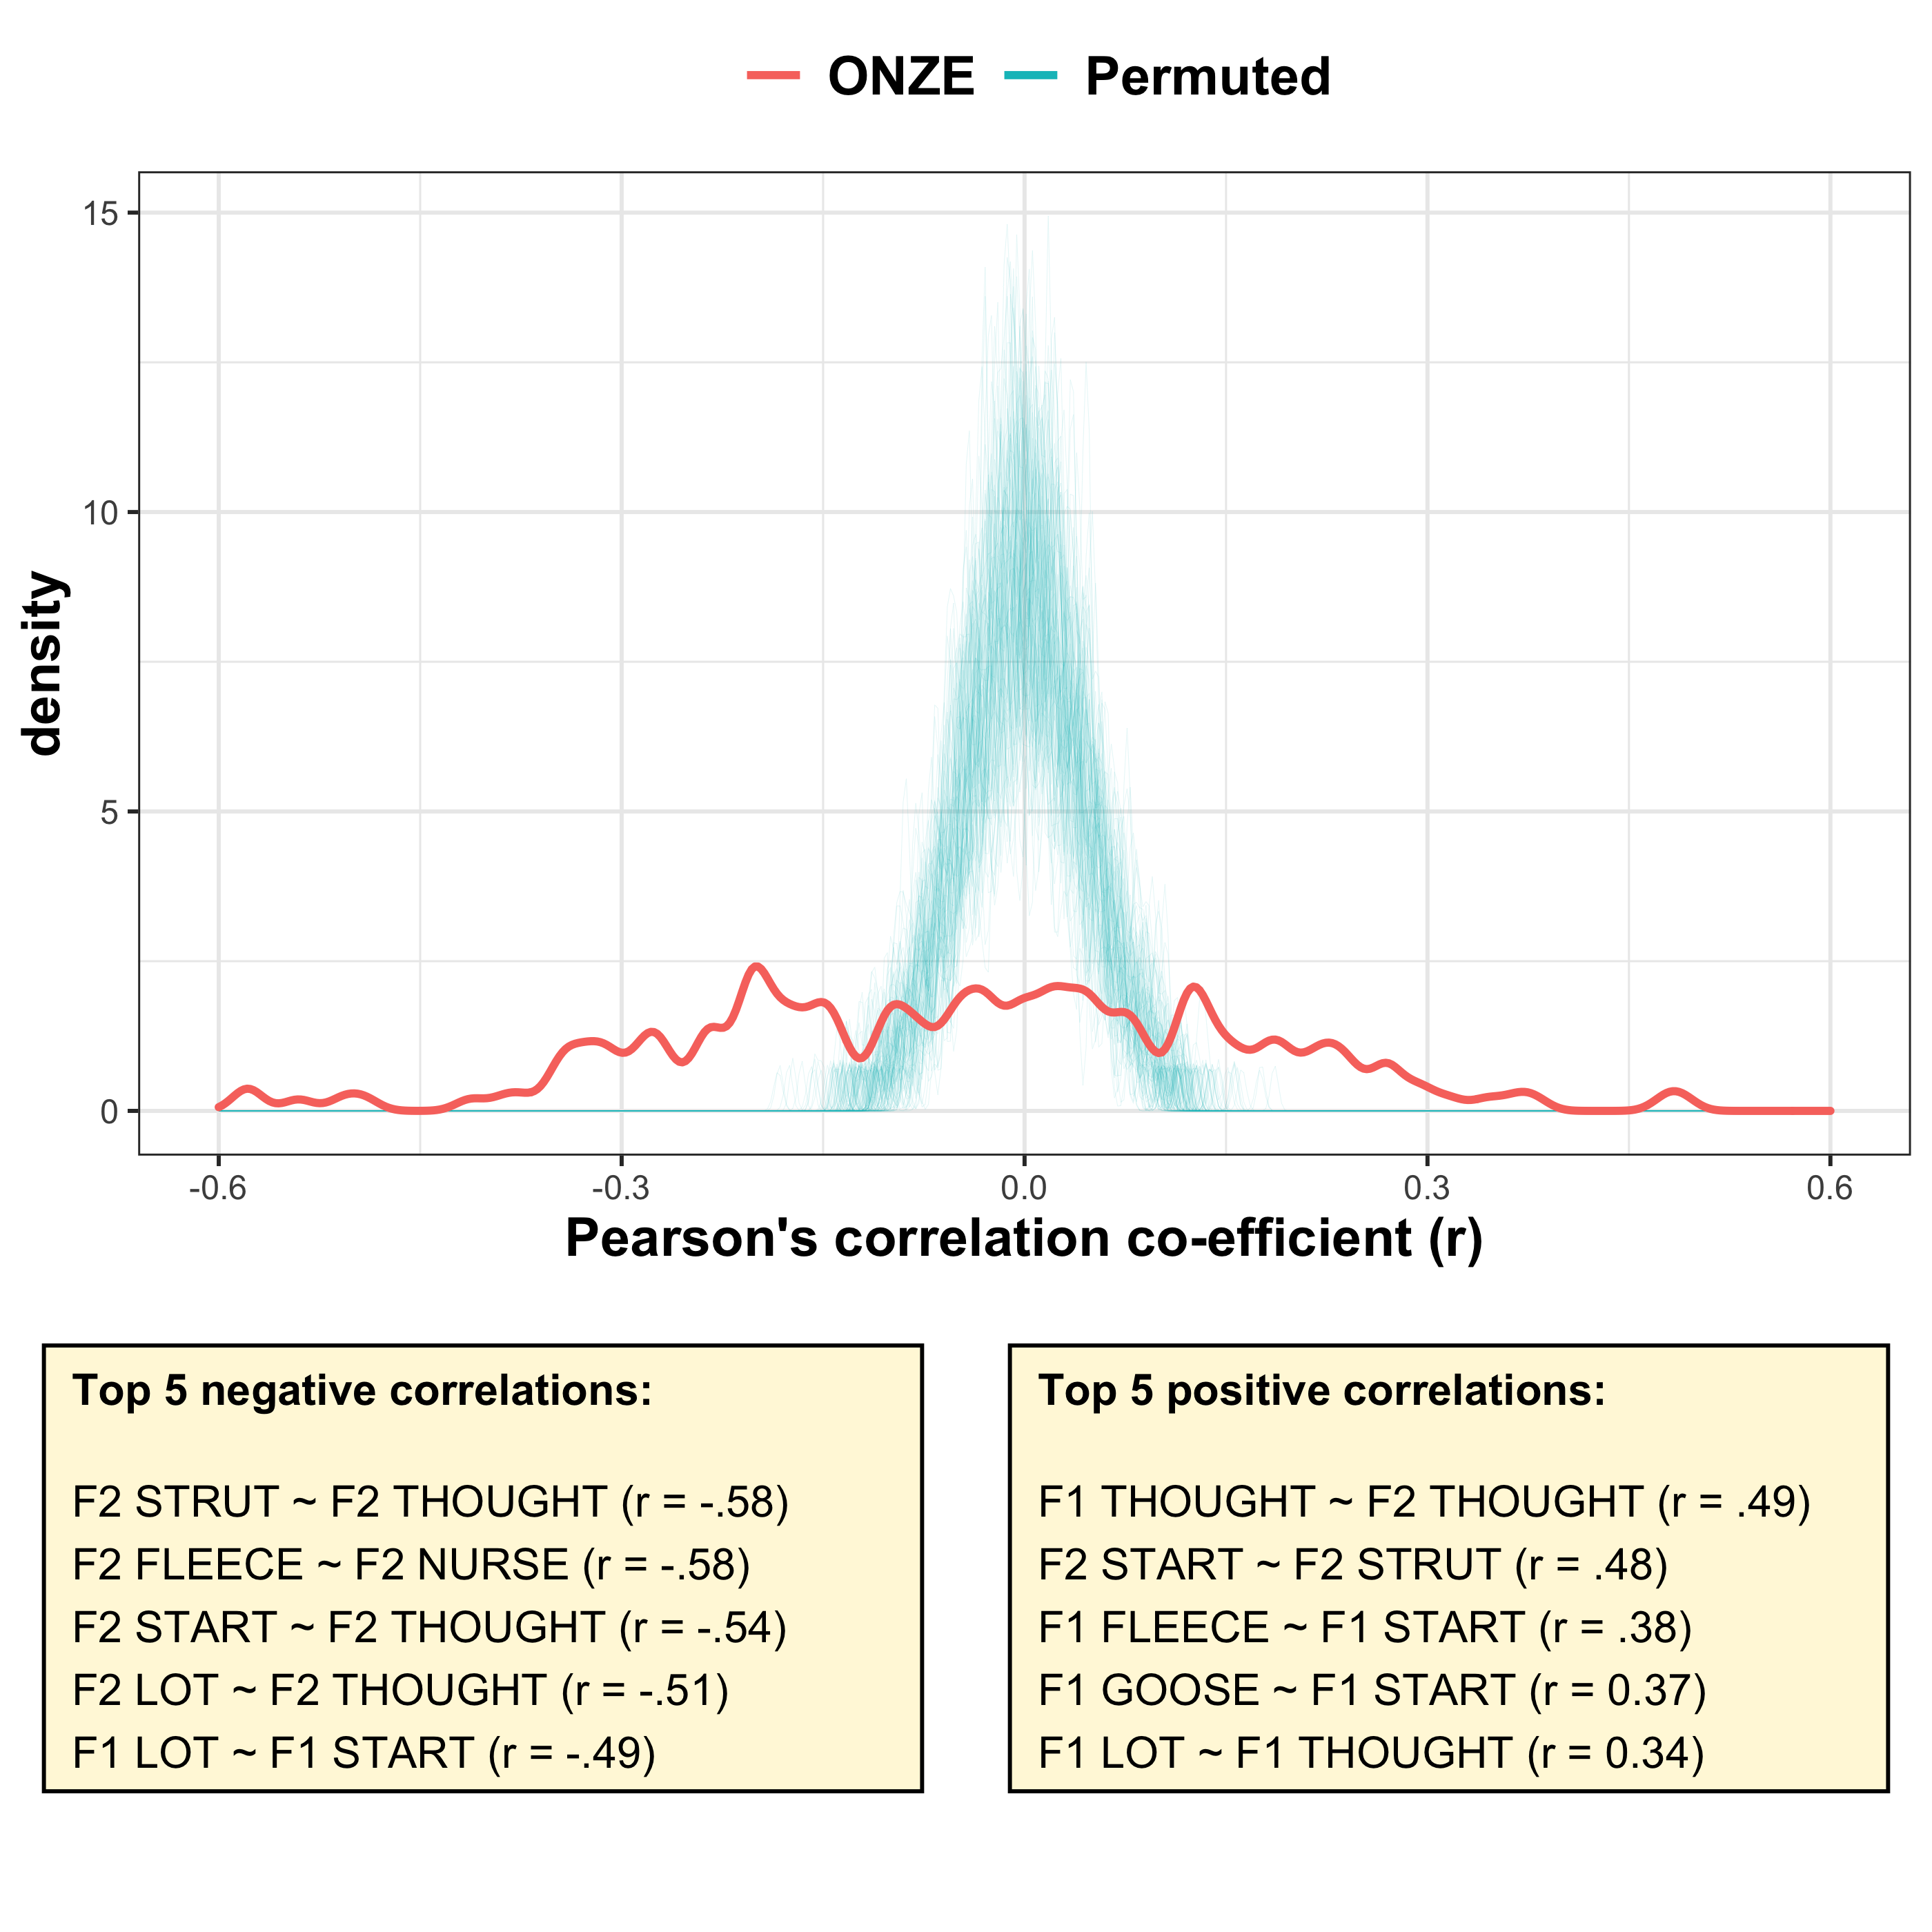
\includegraphics[width=\textwidth]{Figures/correlations_permuted_plot.png}
\caption{Distribution of Pearson correlation co-efficients (r) for the random speaker intercepts extracted from the GAMMs run on the ONZE data (red line), with the five strongest positive and negative correlations given in the boxes below. The distributions where the intercepts have been permuted 100 times are also given (blue lines), which represents what we would expect to find when any underlying structure has been removed.}
\label{fig:correlations}
\end{figure}

%%%%%%%

Our chosen analysis technique to find structure amongst a large set of apparent correlations is Principal Component Analysis (PCA) \citep{venables2013modern, PCAIntro}. We explicitly decided not to rely on simple correlation analyses (as represented in Figure \ref{fig:correlations}) given the large number of variables we are exploring and because we had no strong prior hypotheses regarding which variables will co-vary, making inferential statistics unsuitable for our exploratory analysis. Similarly, we chose not to use clustering algorithms because although they traditionally identify groups of variables that cluster together, the clusters do not necessarily provide insights into the identification of leaders and laggers.   That is, it is difficult to simultaneously interrogate which vowels are covarying (and in which direction), and who the particular speakers are who are positioned at the extreme ends of that co-variation. A cluster analysis may identify a group of speakers leading in a certain subset of variables, another group lagging in the same subset of variables, but it will not be able to provide any link between the two. 
Moreover, a cluster analysis does not offer the multilayered results that PCA does, where independent sources of co-variation can be inspected. Thus, PCA allows for a finer-grained exploration and more theoretically driven interpretation of any co-variation present in the data set, enabling us to not only identify covarying vowels, but identify and visualise specific individuals' vowel spaces that are most responsible for that co-variation.

In addition to the results presented in the following sections, we also offer an interactive web application to explore the results further, accessible at \url{https://onze.shinyapps.io/Covariation_shiny/}. This application allows users to inspect the vowel spaces of each of the 481 speakers, with their individual scores on each of the three PCs, in addition to their demographic information.

\section{Results}

We now present the patterns of sound change as shown by the GAMMs (\ref{sec:soundchange}), and the patterns of co-variation revealed by the PCA (\ref{sec:interpreting}).

\subsection{Patterns of Sound Change}
\label{sec:soundchange}

While our primary purpose in fitting the GAMMs is to control for speaker factors such as year of birth, the major patterns revealed by the GAMMs also facilitate an understanding of sound change occurring over this time period, which is a necessary precursor to interpreting the patterns of co-variation. Figure \ref{fig:sound_change} shows the trajectories of vowel change, based on GAMM smooths over year of birth.  All vowels have undergone some change, either linear or non-linear, based on the year of birth smooth effect (all $p$-values < 0.001), see the Supplementary Materials for the model summaries.  An animated and interactive version of the changes is available in the Shiny application.

%%%%%%%
%sound change
%%%%%%%

\begin{figure}[!t]
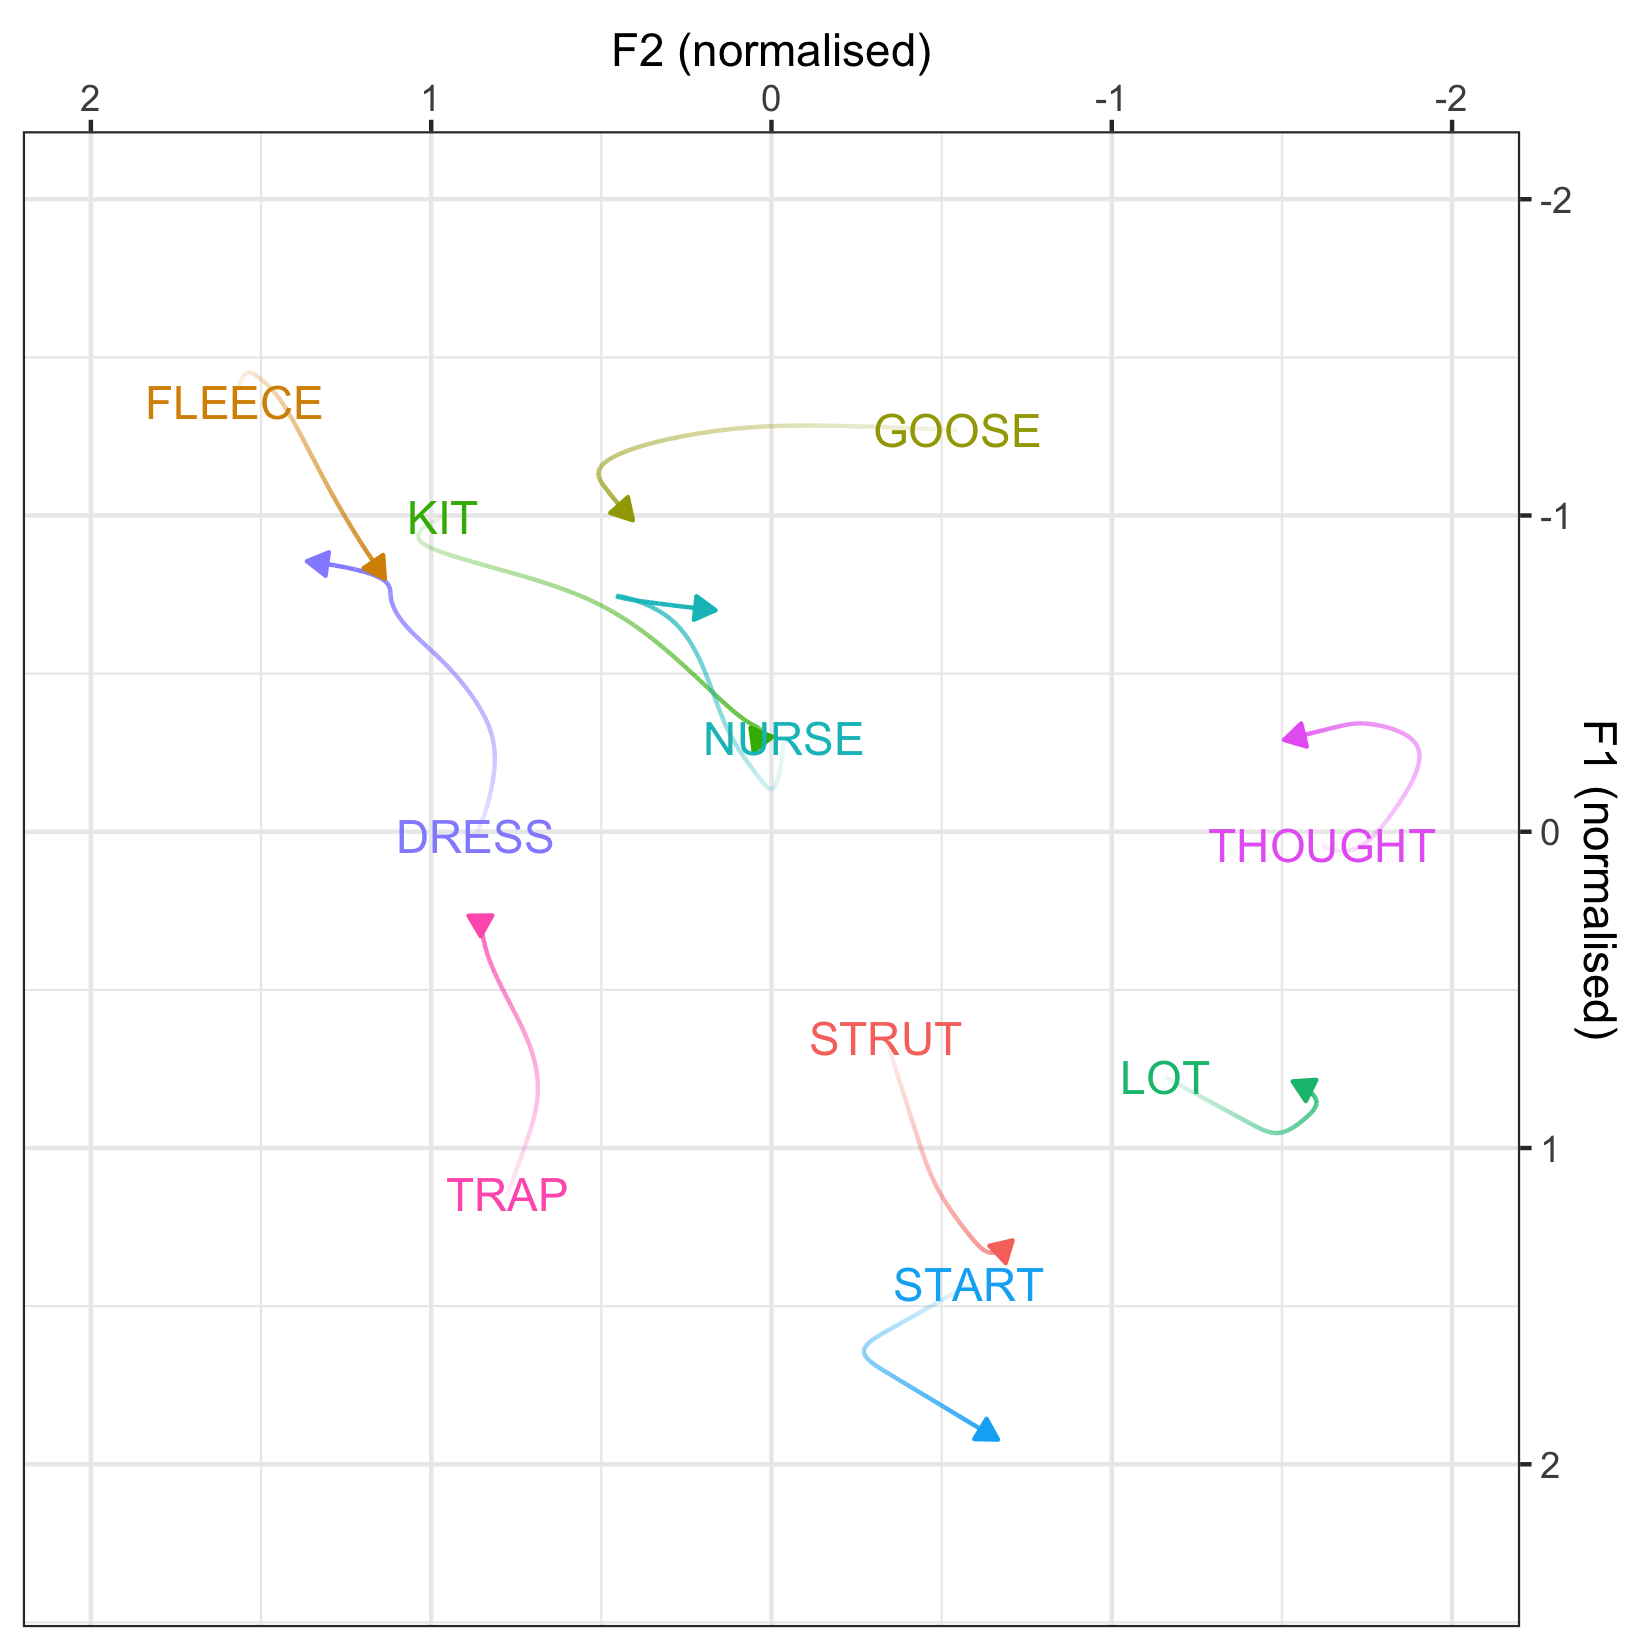
\includegraphics[width=\textwidth]{Figures/sound_change_static.png}
\caption{Trajectories of the 10 vowels based on a GAMM smooth over year of birth. The vowel label represents realisations for speakers born at the start of the ONZE corpus (1864), whereas the end point represents the most recent speakers (1982).}
\label{fig:sound_change}
\end{figure}


\begin{figure}[!t]
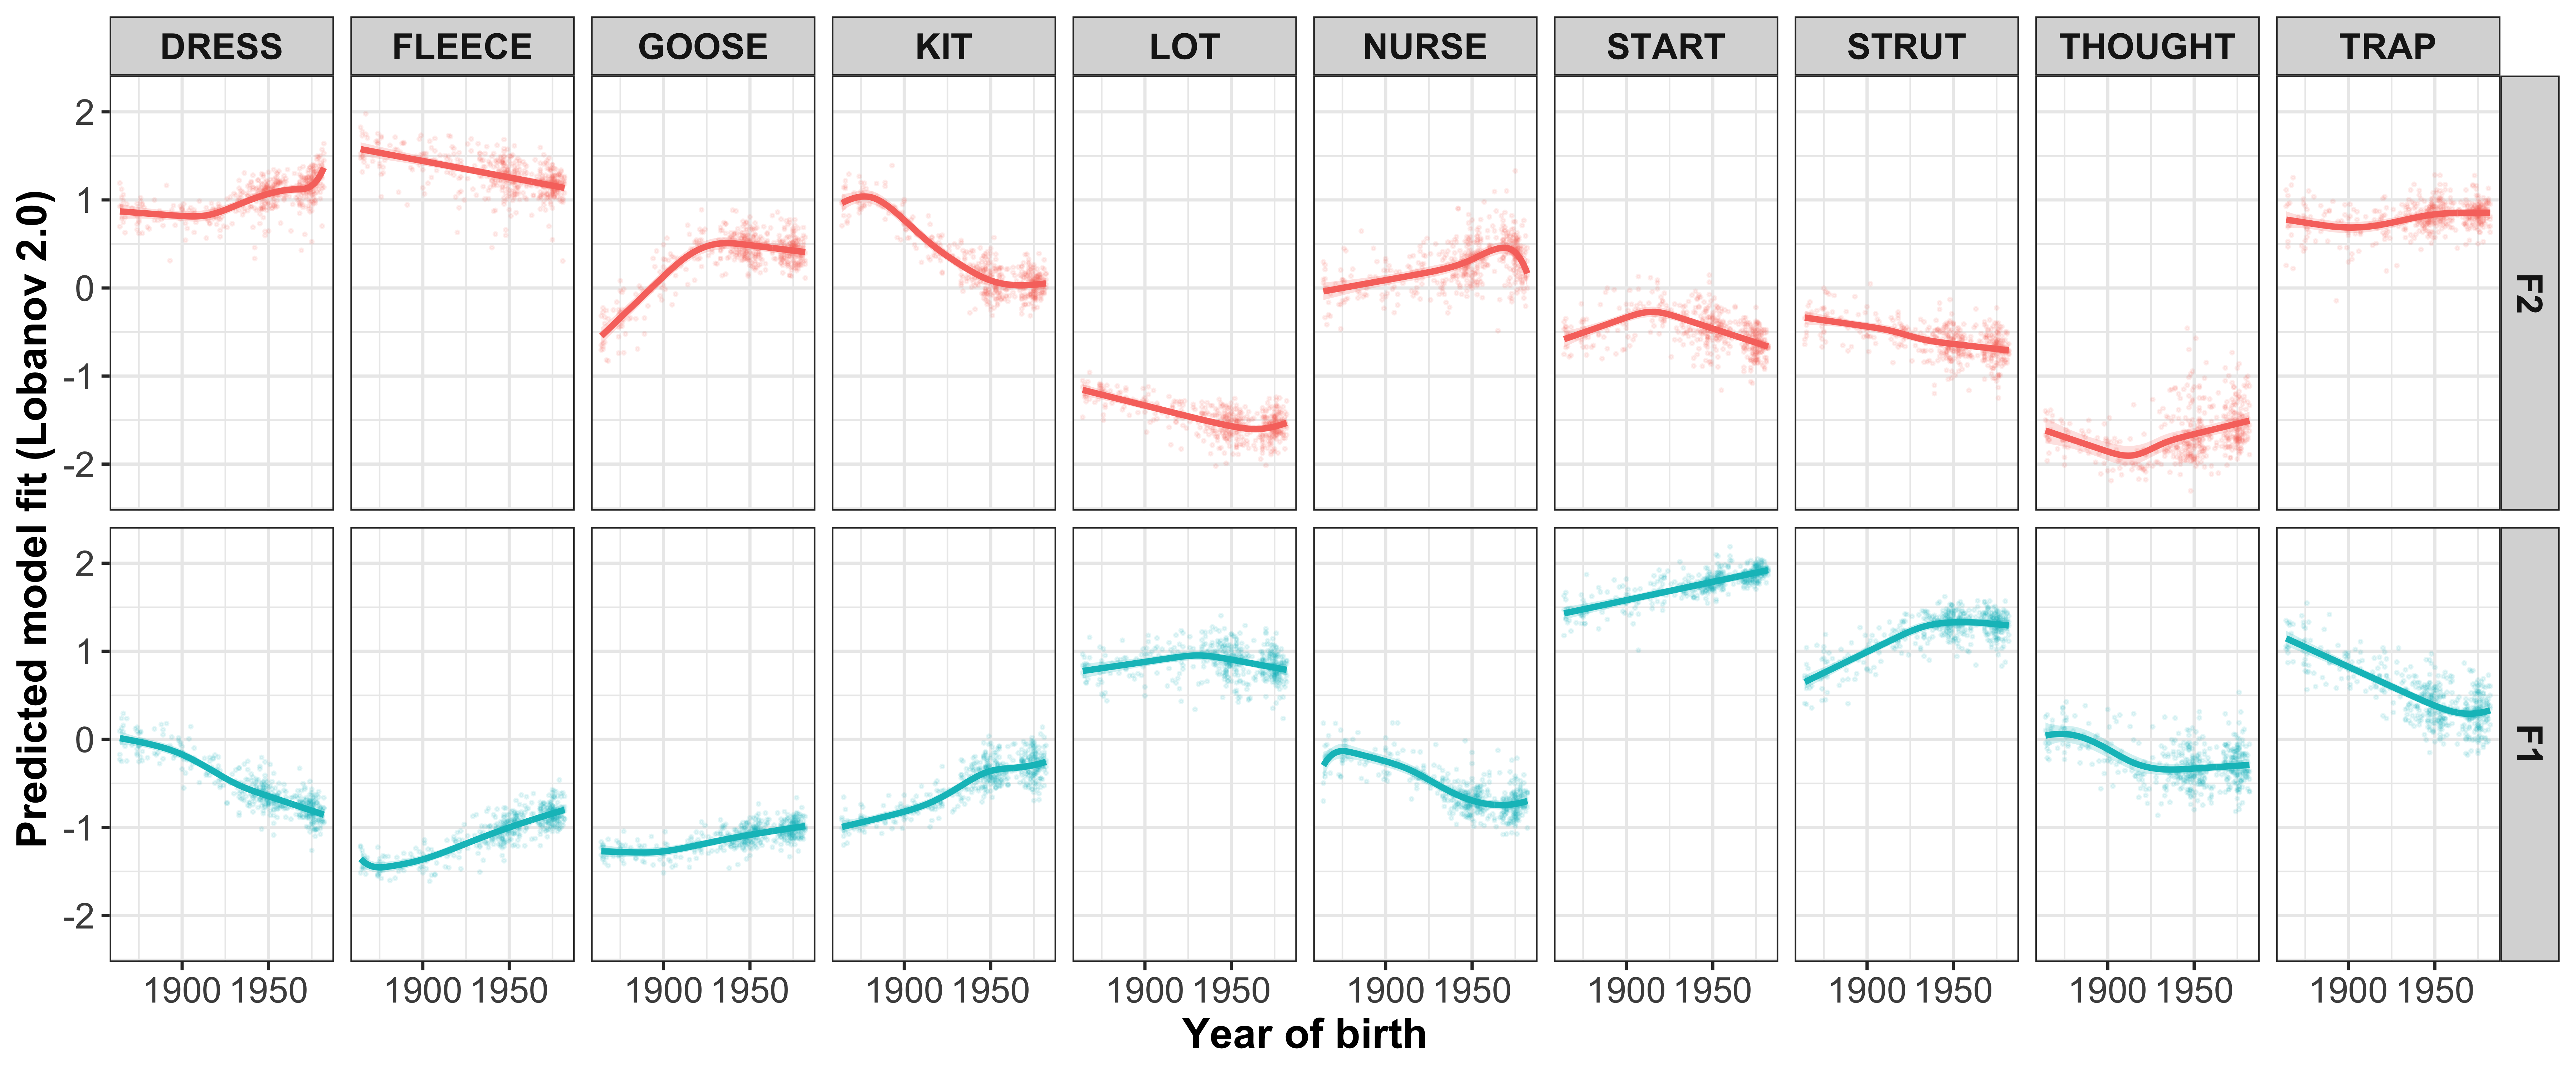
\includegraphics[width=\textwidth]{Figures/sound_change_gam.png}
\caption{Trajectories of vowels based on a GAMM smooth over year of birth (as in figure \ref{fig:sound_change}), with each individual speaker plotted as points around the smooth (calculated by adding their random intercept values to the model fit.}
\label{fig:sound_change_gam}
\end{figure}

The figure shows the well-documented changes of NZE:  raising of \textsc{trap}, \textsc{dress} and centralisation of \textsc{kit}, which are linked together in a chain-shift \citep{hay2015tracking}.  The fronting of \textsc{goose} and the fronting and raising of \textsc{nurse} are also well-documented \citep{maclagan2009u, maclagan2017investigating}.  We also see significant lowering and backing of \textsc{strut}, and that the well-documented early fronting of \textsc{start} \citep{gordon2004new} was followed by a period of considerable backing.  Finally, we see considerable raising of \textsc{thought} and backing of \textsc{lot}.

While the rearrangement of the front short vowels is well-documented, it is relevant to the analysis to also focus on the bottom right quadrant of the vowel space, where the four back vowels start in a diamond shape, with \textsc{thought} and \textsc{start} forming the top and bottom points, and \textsc{strut} and \textsc{lot} sitting adjacent to each other in the middle.
Over time, we then see a gradual rearrangement, into a more `linear' reorganisation in which \textsc{start}, \textsc{strut}, \textsc{lot} and \textsc{thought} are arranged into an elongated linear pattern along the back of the vowel space.   This is achieved, in F1 space, through the lowering of \textsc{strut} and \textsc{start} and the raising of \textsc{thought}.  \textsc{lot} initially slightly lowers, and then raises again. In terms of F2,  \textsc{lot} and \textsc{strut} consistently back, and we see initial fronting of \textsc{start}, followed by considerable backing.  \textsc{thought} shows some initial backing, and then moves frontwards.   

Note that \textsc{thought} and \textsc{strut}, in particular, begin fairly close in height to each other, and then undergo quite dramatic changes in opposing directions. Impressionistically, as \textsc{strut} approaches \textsc{start}, these two vowels appear to move back in tandem, with approximately the same trajectory in F1 and F2 in the latter half of the data.  It is also notable that both \textsc{start} and \textsc{thought} both appear to change direction in F2 movement at about the same time (between 1910 and 1920).  One interpretation may be that the two long vowels were initially repelled by each other (in both F1 and F2), but then once they were sufficiently separated in terms of height, they retreated to their original degrees of backness. The end result of this complex series of changes is a reorganisation in which \textsc{start}, \textsc{strut}, \textsc{lot} and \textsc{thought} are arranged into an elongated linear pattern along the back of the vowel space.   This rearrangement of the back vowels will be discussed further in sections \ref{sec:PC1} and \ref{sec:PC3}.

Importantly, while such trajectories are useful for showing the main direction of change of individual vowels, they conceal considerable individual variation.  Figure \ref{fig:sound_change_gam} shows the same trajectories in vowel-specific panels, this time including points representing the individual speakers alongside the main trend.  This distribution is sometimes very broad, reflecting considerable speaker-based variation around the overall trajectory of change.   The principal components analysis enables us to test whether there is structure in that variation, across vowels.

%nd indicative that not all speakers are necessarily moving in the same direction at the same time. Consider, for example, the F2 of \textsc{nurse}. Towards the end of the trajectory (i.e. the final 10-20 years) the vowel appears to back (decreasing in F2).  However, at the same time, we see an extension of the distribution at this time upwards - a non-trivial number of speakers appearing to continue the previous momentum of \textsc{nurse} fronting.

\subsection{Principal Components Analysis}
\label{sec:interpreting}

As outlined in section \ref{sec:methodology}, the random intercepts from the GAMMs estimate the degree of deviation that individuals show from the main trends of the fixed effect. We therefore used these intercepts as the data in the PCA, allowing us to identify patterns of co-variation that exist across the vowel formants. We will interpret the three most informative principal components (PCs) returned by the PCA, referred to individually as PC1, PC2 and PC3, each of which explain $>$ 10\% of the variance in the data, accounting for 43.1\% of the variance overall. Each PC identifies distinct sources of co-variation in the data set, which can be understood by assessing which vowel-specific formants are explaining the most variation in the PC. 

We will describe for each PC:

\begin{itemize}

    \item \textit{Which} specific vocalic variables load meaningfully onto the PC (determined by the contributions made by each variable).
    
    \item \textit{What} this tells us about the way certain vocalic variables are realised by different speakers in terms of the F1$\sim$F2 space.
    
    \item \textit{If} the PC can be explained by demographic factors such as year of birth or gender.
    
\end{itemize}

We first note that the signs of the PCs in a PCA solution are completely arbitrary. For instance, if there was a PC corresponding to leaders \textit{versus} laggers in multiple changes, it could be coded such that leaders are assigned positive scores and laggers negative scores; but it could also be coded the opposite way, with leaders receiving negative scores and laggers positive scores. The two PCA solutions are mathematically equivalent.

The {\em PC loadings} that the PCA assigns to each of the vowel formants indicate how important each vowel formant is to each PC, and also provide information about their directionality. The directions of the loadings can be interpreted in terms of their sign ($+/-$) within the context of the wider PC. Given the arbitrariness of the signs of the PC scores, the loading directions in themselves are not meaningful. However, the way these signs pattern together across different vowel specific formants is potentially meaningful. If the signs are the same for any pair of formants (e.g.\ both are positive) then it indicates that they are co-varying in the same direction, whereas if the signs contrast (e.g.\ a positive and a negative) then it indicates that the formants are co-varying in opposite directions.

Similarly, each of the speakers in the dataset is assigned a {\em PC score} for each component. This value indicates the extent to which a given speaker exhibits the pattern of co-variation in a given PC. Again, these can be interpreted in terms of $+/-$ signs, which are arbitrarily assigned. Speakers with large absolute PC scores are at the margins of the co-variation. Any speaker with a large positive score would be interpreted as co-varying in one direction, while a speaker with a large negative score will be co-varying in the opposite direction. It is through the combination of the PC loadings and the PC scores that we can determine whether we can observe `leaders' and `laggers' of sound change, or other forms of co-variation.

%%%%%%%

\subsubsection{PC1: The restructuring back vowels}
\label{sec:PC1}

%%%%%%%
%PC1_variable_loadings
%%%%%%%

% \begin{figure}[!ht]
% \includegraphics[width=\textwidth]{Figures/PC1_plot_variables_combined.png}
% \caption{\textbf{A} Dot plot of the contributions of each vowel formant from PC1, the larger the contribution the more variance explained and therefore the more important that vowel formant is to the PC. The contributions are calculated by squaring the vowel formant loading. vowel formants that are to the right of the red dashed line collectively contribute over 50\% to the PC. The $+/-$ signs indicate the direction of the loadings. \textbf{B} Visualisation of how the loadings can be interpreted in terms of F1$\sim$F2 space. The location of the vowel label indicates the position of realisations made by speakers with low scores on PC1, with the trajectory ending at the position where speakers with highest scores are (based on GAMM smoothing). The size of the vowel label is indicative of the importance of the vowel to PC1.}
% \label{fig:PC1_variable_loadings}
% \end{figure}

%%%%%%%

PC1 accounted for 17.2\% of the total variance in the PCA.  Figure \ref{fig:PC1_variable_loadings}A shows the contributions made by each vowel formant to the PC. To help with the interpretation of which vowel formants are most important to the PC, we present the contributions as a contribution percentage. These are calculated by squaring the individual loadings and then multiplying them by 100, to give a value that represents how much the vowel formant contributes to the variance explained by the PC (see \citealt{PCAIntro}).  The vowel formants are ordered left to right as a function of their contribution percentage. There is a clear cluster of four variables which drive this PC: \textsc{thought} F1 and F2, and the F2 of \textsc{start} and \textsc{strut}, all of which collectively contribute over 50\% to the PC (i.e.\ are to the right of the red dashed line). Each vowel formant has a positive or negative sign, which indicates the directional relationship of the co-variation between all of the other vowel formants. For instance, \textsc{thought} F2 is negative (red `$-$' sign in Figure \ref{fig:PC1_variable_loadings}A), indicating that speakers with a low PC1 score will have a more backed \textsc{thought} realisation, i.e. their F2 values are low. Conversely, \textsc{strut} is positive (black `$+$' sign), indicating that the co-variation is operating in the opposite direction, i.e. speakers with a low PC1 score will have a fronter \textsc{strut} realisation.\footnote{Note again that the $+/-$ signs are arbitrary in the sense that if all of the signs are reversed, the interpretation will remain the same.}

\begin{figure}[!p]
\includegraphics[width=\textwidth]{Figures/PC1_plot.png}
\caption{\textbf{A} Dot plot of the contributions of each vowel formant from PC1, the larger the contribution the more variance explained and therefore the more important that vowel formant is to the PC. Vowel formants that are to the right of the red dashed line collectively contribute over 50\% to the PC. The $+/-$ signs indicate the direction of the loadings. \textbf{B} Visualisation of how the loadings can be interpreted in terms of F1$\sim$F2 space. The location of the vowel label indicates the position of realisations made by speakers with the lowest PC1 scores, with the trajectory ending at the position where speakers with the highest scores are. The size and colour of the vowel label is indicative of the importance of the vowel to PC1. \textbf{C} The trajectories of change for each vowel formant by year of birth (red line), with the speaker intercepts plotted as points around the trajectory. The colour of the points indicates the speaker's PC score, where green points are positive scores and black are negative. The contribution percentages for each vowel formant are given at the top of the panels and the most important vowel formants are highlighted by yellow boxes.}
\label{fig:PC1_variable_loadings}
\end{figure}


PC1 relates to the overall position of \textsc{thought}, and to the F2 of \textsc{start} and \textsc{strut} - all vowels involved in the linear reorganisation of the back vowels as discussed in section \ref{sec:soundchange}.  Several visualisations help us interpret the PC.  First, in Figure \ref{fig:PC1_variable_loadings}B, we see the trajectory from speakers with the lowest PC1 score to those with the highest PC1 score.  These trajectories are the fitted values from linear regressions predicting the speaker intercepts by the speaker's PC1 scores. These are used for visualisation purposes, in order to give an impression of the degree and directionality of the loadings in terms of F1$\sim$F2 space.  They illustrate the distribution of speakers from low PC1 (in black) to high PC1 (in green), and show that high PC1 speakers have backer \textsc{start} and  \textsc{strut} vowels, and lower, fronter \textsc{thought}. 

% are smooths derived from GAMMs that predict the normalised F1/F2 values in our dataset (as was the case for the initial GAMM modelling), but here we use a fixed effect of PC1 score as the fixed effect predictor. The arrows give us information about the degree of variation involved, and the direction of the loading.\footnote{We do not provide any model summaries of these GAMMs as we are only using them to assist in the interpretation of the PC. Given that NZE has also undergone various sound changes (see Section \ref{sec:PC2}), there is considerable variation in the realisations of vowels across time, therefore the location of the vowels in Figures \ref{fig:PC1_variable_loadings}, \ref{fig:PC2_variable_loadings} and \ref{fig:PC3_variable_loadings} masks over year of birth differences.}

%%%%%%%
% The relevant GAMM smooths are also shown in Figure \ref{fig:PC1_yob}, overlaid on the same plots as the corresponding sound change trajectories - normalized formant values plotted by year of birth (as in Figure \ref{fig:sound_change_gam}).
In Figure \ref{fig:PC1_variable_loadings}C we can see how the speaker intercepts from the sound change models relate to the speaker PC scores. When the positive and negative scores (green and black points respectively) are clearly distinguishable above and below the sound change smooth (red line), this indicates that the degree of co-variation is large (with the yellow outlines used to highlight which vowel formants contribute most to the PC). This also aids in the assessment of whether the loadings are aligned in the same direction of sound change (separating, for example `leaders' and `laggers' of a constellation of changes) or whether they are pushing in somewhat separate directions.  In a sound change trajectory showing a positive slope for example, 'leaders' will appear above the smooth line.  If these points appear systematically green, then high PC1 speakers are systematically leading for that change.

In this visualisation we see again that speakers with high PC1 scores have considerably larger F1 and F2 intercepts for \textsc{thought}, that is, their \textsc{thought} is lower and fronter in comparison to the rest of the population.
Speakers with high PC1 scores have lower F2 intercepts (are backer) for \textsc{start} and \textsc{strut} than the rest of the population.

How does this compare to the direction of sound change?  The answer is straightforward for \textsc{strut} F2 and \textsc{thought} F1, both of which show a consistent direction of change.  Speakers with high PC1 scores are innovative for the backing of \textsc{strut} and conservative for the raising of \textsc{thought}.  In other words, speakers who are leaders in one of these sound changes tend to be laggers in the other. Some speakers participate in the linear reorganisation of the back vowels by raising \textsc{thought}, and remaining conservative for \textsc{strut}, whereas a different set of speakers participate by innovatively lowering \textsc{strut}, and remaining conservative for \textsc{thought}.

\textsc{start} and \textsc{thought} F2 are more complex to interpret because they begin by moving away from each other (with \textsc{start} fronting and \textsc{thought} backing), and then start to move back towards each other. Speakers with high PC1 scores have a backer \textsc{start} F2, and thus would be conservative for early speakers, but innovative for later speakers.  Similarly, those same speakers have fronter \textsc{thought} F2, and thus would be conservative for early speakers, but innovative for later speakers.

Innovation in F2 for \textsc{start} and \textsc{thought} does not mean the same thing for early and late speakers, but in both cases the vowels are linked together.   For earlier speakers, innovation in \textsc{start/thought}  F2 is associated with speakers who are less innovative in \textsc{strut}-backing and more innovative in \textsc{thought}-raising.  For later speakers, it is associated with those speakers who are more innovative in \textsc{strut}-backing, and less innovative in \textsc{thought}-raising.

To summarise, as \textsc{strut} backs, \textsc{thought} raises.  These changes are linked, such that if an individual speaker was leading in one change, they were likely to be lagging in the other. In early NZE, those who were advanced in \textsc{thought} raising were also backing \textsc{thought}, while fronting \textsc{start}.  By around 1910-1920, \textsc{thought} was relatively high, and started to front again, while \textsc{start} appears to have become linked with  \textsc{strut}, and backed in parallel with it.  The same speakers led both \textsc{thought}-fronting and \textsc{start}-backing, and they were the same speakers who were advanced at this time in the backing of \textsc{strut}.   




Pairwise correlations (see Figure \ref{fig:correlations} and the \hyperref[sec:supplementarymaterials]{Supplementary Materials}), show that the strongest `link' amongst the top 4 variables in PC1 are a negative correlation between \textsc{strut} and \textsc{thought} F2 ($r = -.58$). There is also a strong positive link between \textsc{strut} and \textsc{start} F2 ($r = .48$). This reinforces the interpretation that PC1 is carried by a repulsive relationship between \textsc{thought} and \textsc{strut}, together with a link between the front/back dimension of \textsc{strut} and \textsc{start}. Likewise, we observe a strong negative link between \textsc{thought} F1 and F2 ($r = -.54$), highlighting that when \textsc{thought} is lower, it is also likely to be backer.


In sum, we have a set of three vowels that move in a complex but co-ordinated fashion over the time period.  At any given time, if we know the position of one of the vowels for a speaker, we can make a reasonable estimation of the position of the other two.  Vowels in the system appear to be linked both through repulsion (e.g. \textsc{thought} and \textsc{start/strut} for early speakers), and through potential structural association (in the case of \textsc{start/strut} for the later speakers).



\begin{figure}[!t]
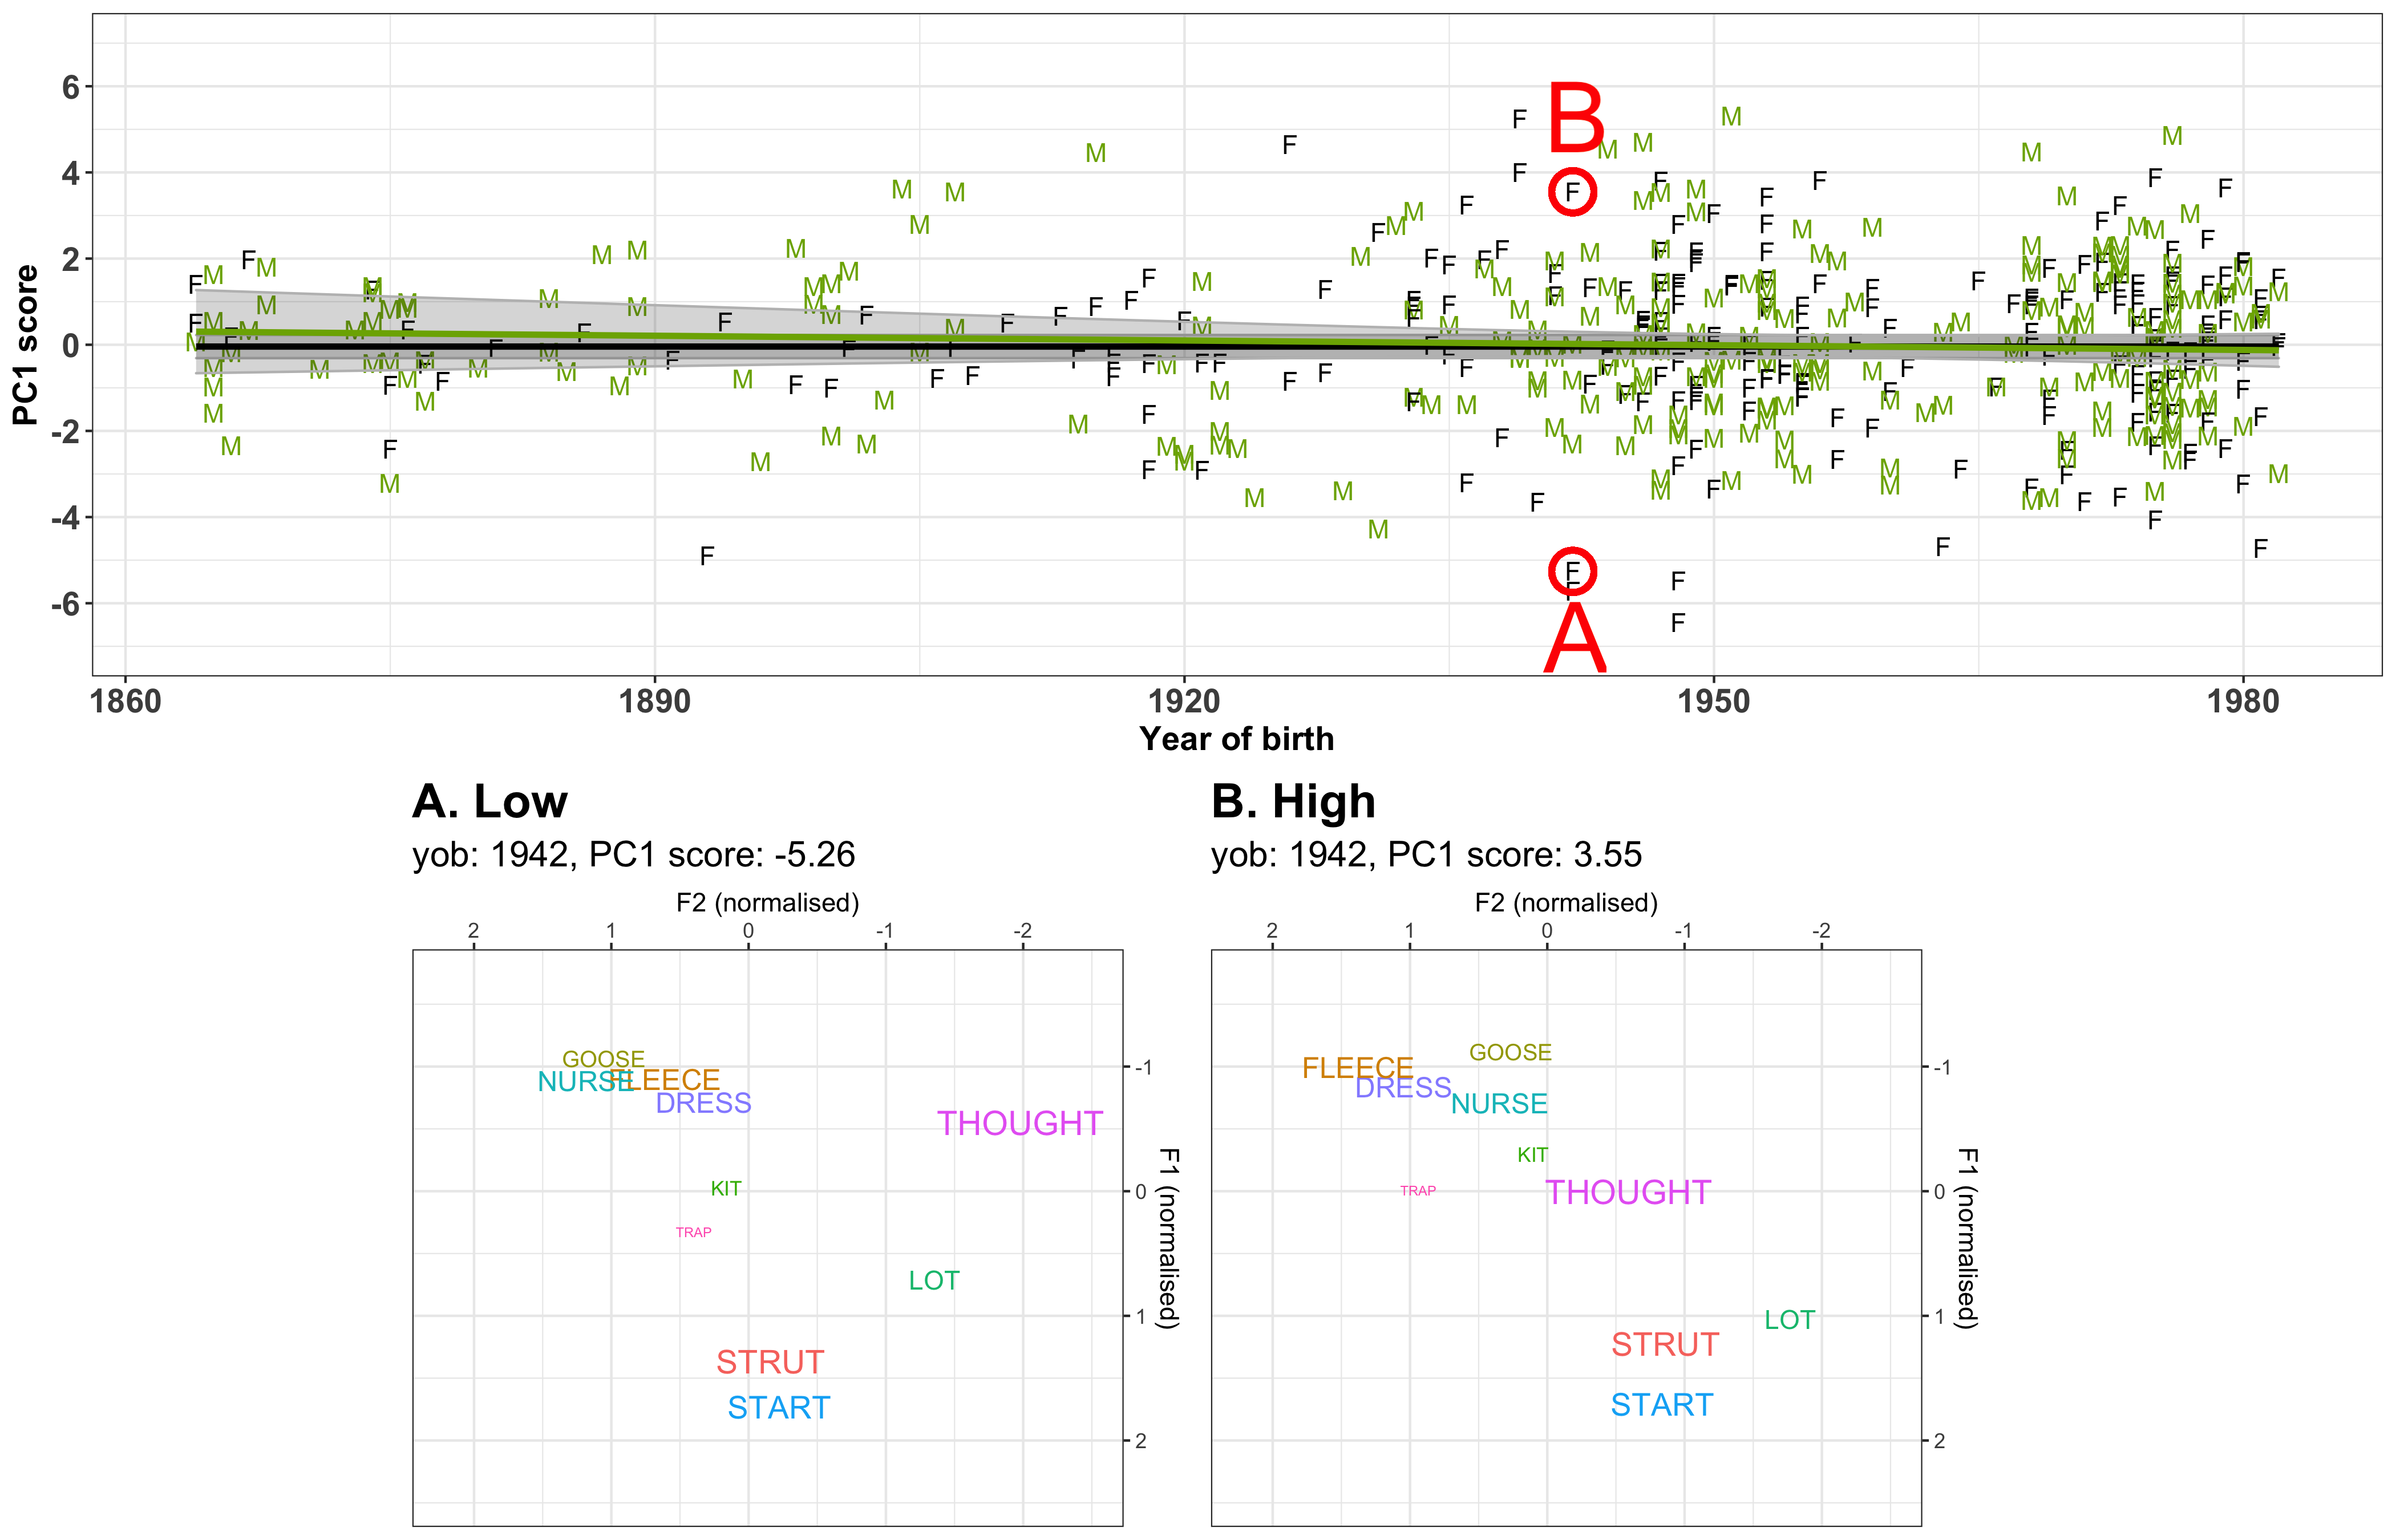
\includegraphics[width=\textwidth]{Figures/PC1_speaker_loadings_example.png}
\caption{\textbf{Top panel} Relationship between year of birth and speaker PC scores for PC1. Each black F and green M (for female and male speakers respectively) indicates an individual speaker in the data set. Two GAM smooths are fitted (green and black lines), highlighting the lack of relationship between year of birth and PC1 score for both genders. \textbf{Bottom panel} Two speakers of the same gender and similar year of birth have been circled to represent a negative (speaker \textbf{A}) and a positive PC score (speaker \textbf{B}), with their vowel spaces given in the bottom panel.}
\label{fig:PC1_speaker_loadings}
\end{figure}

As shown in Figure \ref{fig:PC1_speaker_loadings} (top panel), these patterns of co-variation exist across speakers even when we control for year of birth and gender.  At any given time there are speakers who are `high PC1' speakers, and those who are `low PC1' speakers, with the PC score indicating where they sit for this set of relationships, given their year of birth.  In Figure \ref{fig:PC1_speaker_loadings} (bottom panel) we also see examples of vowel spaces from speakers born at the same time - in the later part of the sound change - with low and high PC1 scores. Their vowel spaces are plotted in  A (a low PC1 speaker) and B (a high PC1 speaker).  In terms of the linear reorganisation of the back vowels, speaker A is advanced in the raising of \textsc{thought}, but still has relatively front \textsc{strut}/\textsc{start}, and \textsc{thought} has not yet fronted.   Speaker B has more innovative backer \textsc{strut/start}, and \textsc{thought} is front, but is correspondingly less raised.  Comparing across the speakers, we see that the degree of backness of \textsc{strut}/\textsc{start} is comparable.  In the most general terms, we can say that speakers with high PC1 scores are innovative in F2 for this cluster of three vowels, and conservative in F1 (for \textsc{thought}) .  Speakers with low PC1 scores show the opposite pattern.

\subsubsection{PC2: `leaders' and `laggers' of sound change}
\label{sec:PC2}

%%%%%%%
%PC2_variable_loadings
%%%%%%%

% \begin{figure}[!ht]
% \includegraphics[width=\textwidth]{Figures/PC2_plot_variables_combined.png}
% \caption{\textbf{A} Dot plot of the contributions of the vowel formants to PC2.The most important vowel formants are shown the right of the red dashed line, which together contribute over 50\% to the PC. \textbf{B} Visualisation of how the loadings can be interpreted in terms of F1$\sim$F2 space. The location of the vowel label indicates the position of realisations made by speakers with low scores on PC2, with the trajectory ending at the position where speakers with high scores are (based on GAMM smoothing). The size of the vowel label is indicative of the importance of the vowel to PC2.}
% \label{fig:PC2_variable_loadings}
% \end{figure}

%%%%%%%

The second PC accounted for 15.8\% of the total variance. Figure \ref{fig:PC2_variable_loadings}A gives the contributions for each of the vowel formants, in addition to a visualisation of how these can be interpreted in terms of F1$\sim$F2 space (\ref{fig:PC2_variable_loadings}B). We see that the highest contributor is \textsc{trap} F1.  This is plotted with a black `$+$' sign, indicating it is positively loaded onto PC2, meaning that speakers with high PC2 scores have a raised \textsc{trap}. \textsc{fleece} F1, on the other hand, is negatively loaded onto PC2, which is plotted with a red `$-$ sign, indicating a negative loading.  In other words, speakers with a high PC2 score have a low F1 \textsc{fleece}. While \textsc{trap} F1 is particularly strongly implicated in PC2, unlike for PC1, there is no leading cluster of variables driving the PC.  We concentrate on the set of variables with the highest contribution to PC2 which cumulatively explain > 50\% of co-variation (i.e. to the right of the red dashed line). Figure \ref{fig:PC2_variable_loadings}B gives a visual representation of the directionality of the vowel formants in F1$\sim$F2 space, as we move from speakers with low to high PC scores. Figure \ref{fig:PC2_variable_loadings}C again shows the trajectories of sound change for each of the vowel formants, with the individual speaker intercepts plotted around the trajectory, speakers with high/low PC2 scores are plotted in green/black respectively.

\begin{figure}[!p]
\includegraphics[width=\textwidth]{Figures/PC2_plot.png}
\caption{\textbf{A} Dot plot of the contributions of each vowel formant from PC2, the larger the contribution the more variance explained and therefore the more important that vowel formant is to the PC. vowel formants that are to the right of the red dashed line collectively contribute over 50\% to the PC. The $+/-$ signs indicate the direction of the loadings. \textbf{B} Visualisation of how the loadings can be interpreted in terms of F1$\sim$F2 space. The location of the vowel label indicates the position of realisations made by speakers with the lowest PC2 scores, with the trajectory ending at the position where speakers with the highest scores are. The size and colour of the vowel label is indicative of the importance of the vowel to PC2. \textbf{C} The trajectories of change for each vowel formant by year of birth (red line), with the speaker intercepts plotted as points around the trajectory. The colour of the points indicates the speaker's PC score, where green points are positive scores and black are negative. The contribution percentages for each vowel formant are given at the top of the panels and the most important vowel formants are highlighted by yellow boxes.}
\label{fig:PC2_variable_loadings}
\end{figure}

% \begin{figure}[!ht]
% \includegraphics[width=\textwidth]{Figures/PC2_yob_important.png}
% \caption{GAMM smooths for vowel formants contributing to co-variation captured by PC2. Dotted lines show the trajectory of the formant over time -- from earlier born to later born speakers, for F1 (red) and F2 (blue) respectively.  Solid lines overlay the trajectory of the formants from speakers with low to high PC2 scores.}  
% \label{fig:PC2_yob}
% \end{figure}

In the case of PC2, there is complete alignment with sound change. We therefore interpret PC2 as highlighting co-variation in terms of vowels known to have undergone significant sound changes in NZE. If speakers are ahead in one of these changes, they are likely to be ahead in all of them.  We can see that the well documented short front vowel shift is reflected in the PC, with F1 for \textsc{trap} and \textsc{dress} both lowering (vowels raising), and \textsc{kit} F2 lowering (vowel backing). Further to this, the PC also captures movement of \textsc{nurse} and \textsc{fleece} in the direction of change over time, as well as the back vowel \textsc{lot}. This indicates that there is co-variation of a specific constellation of vowels that represent differences in speakers being advanced, or behind, in the evolving sound system. We see this as identifying `leaders' and `laggers' of sound change -- at any point in time there are speakers whose realisations are already advancing towards the direction of change. Moreover, this also shows that there are certain speakers who are in the opposite direction of change, those who are conservative in this cluster of sound changes and who are lagging behind.  Indeed, if we continue down below the 50\% contribution line, we find that the next five vowels are also loaded in the same direction as sound change -- we need to go down to F2 \textsc{thought} (the 12\textsuperscript{th} highest contributor to the PC) to find a vowel that is not aligned.

An inspection of the speaker's PC2 scores in the top panel of Figure \ref{fig:PC2_speaker_loadings} reveals that there is no significant relationship between year of birth and whether you are a `leader' (high positive PC2 score) or a `lagger' (large negative PC2 score), with the same being true for gender. Crucially, this shows that our GAMMs were able to control for the known predictors of sound change included in the models (specifically, year of birth and gender), giving us confidence that this modelling step has factored out such sources of known co-variation. Furthermore, the fact that there are speakers with large absolute scores (both positive and negative) across the time period demonstrates that at any point in time there will likely be speakers who are leading and lagging in sound changes, not just for a single variable, but for a sub-system of variables.

In the top panel of Figure \ref{fig:PC2_speaker_loadings}, we can see the `leaders' and `laggers' (those who have large positive/negative PC2 scores), but we can also see those speakers with scores close to zero: these are speakers who are exactly where we expect them to be with respect to this set of vowels given their birth year. In other words they are the speakers who are typical of the population for that point in time. Shown in the bottom panel of Figure \ref{fig:PC2_speaker_loadings} are vowel spaces from four example speakers, which illustrate the type of co-variation that the PC captures. Speakers A and D are two typical speakers born 40 years apart (both males with PC2 scores close to zero).  As would be expected, their vowel spaces are substantially different. Of particular note is D's raising of \textsc{nurse}, backing of \textsc{lot}, and general progression in the short front vowel shift. Speakers B and C are both males who are born at the midpoint between speakers A and D, with birth dates that are very close together. C has a positive PC2 score, and so is more advanced than we would expect for the vowels implicated in PC2, so is considered to be a `leader'.  B has a negative PC2 score, and so is less advanced than we would expect, so is considered to be a `lagger'.  Visual comparison of the vowel spaces reveals that, although speakers B and C share similar years of birth, the `lagger' looks a lot like the older speaker (A), and the `leader' looks a lot like the younger speaker (D). In other words, moving from a speaker with a low PC2 score to a speaker with a high PC2 score appears to be roughly equivalent to moving between speakers (with a PC2 score of $\sim$0) who are born 40 years apart.\footnote{Note that comparing speakers with high and low PC2 scores to speakers born earlier and later is relatively straightforward for this PC, because all of the vowels are loaded in a direction that is aligned with the directions of ongoing sound change.  It would be more difficult for the other PCs, neither of which show this complete alignment with ongoing sound changes. The online Shiny application allows exploration of the vowel spaces for all speakers in the data set for the three main PCs.}

%%%%%%%
%PC2_speaker_loadings
%%%%%%%

\begin{figure}[!t]
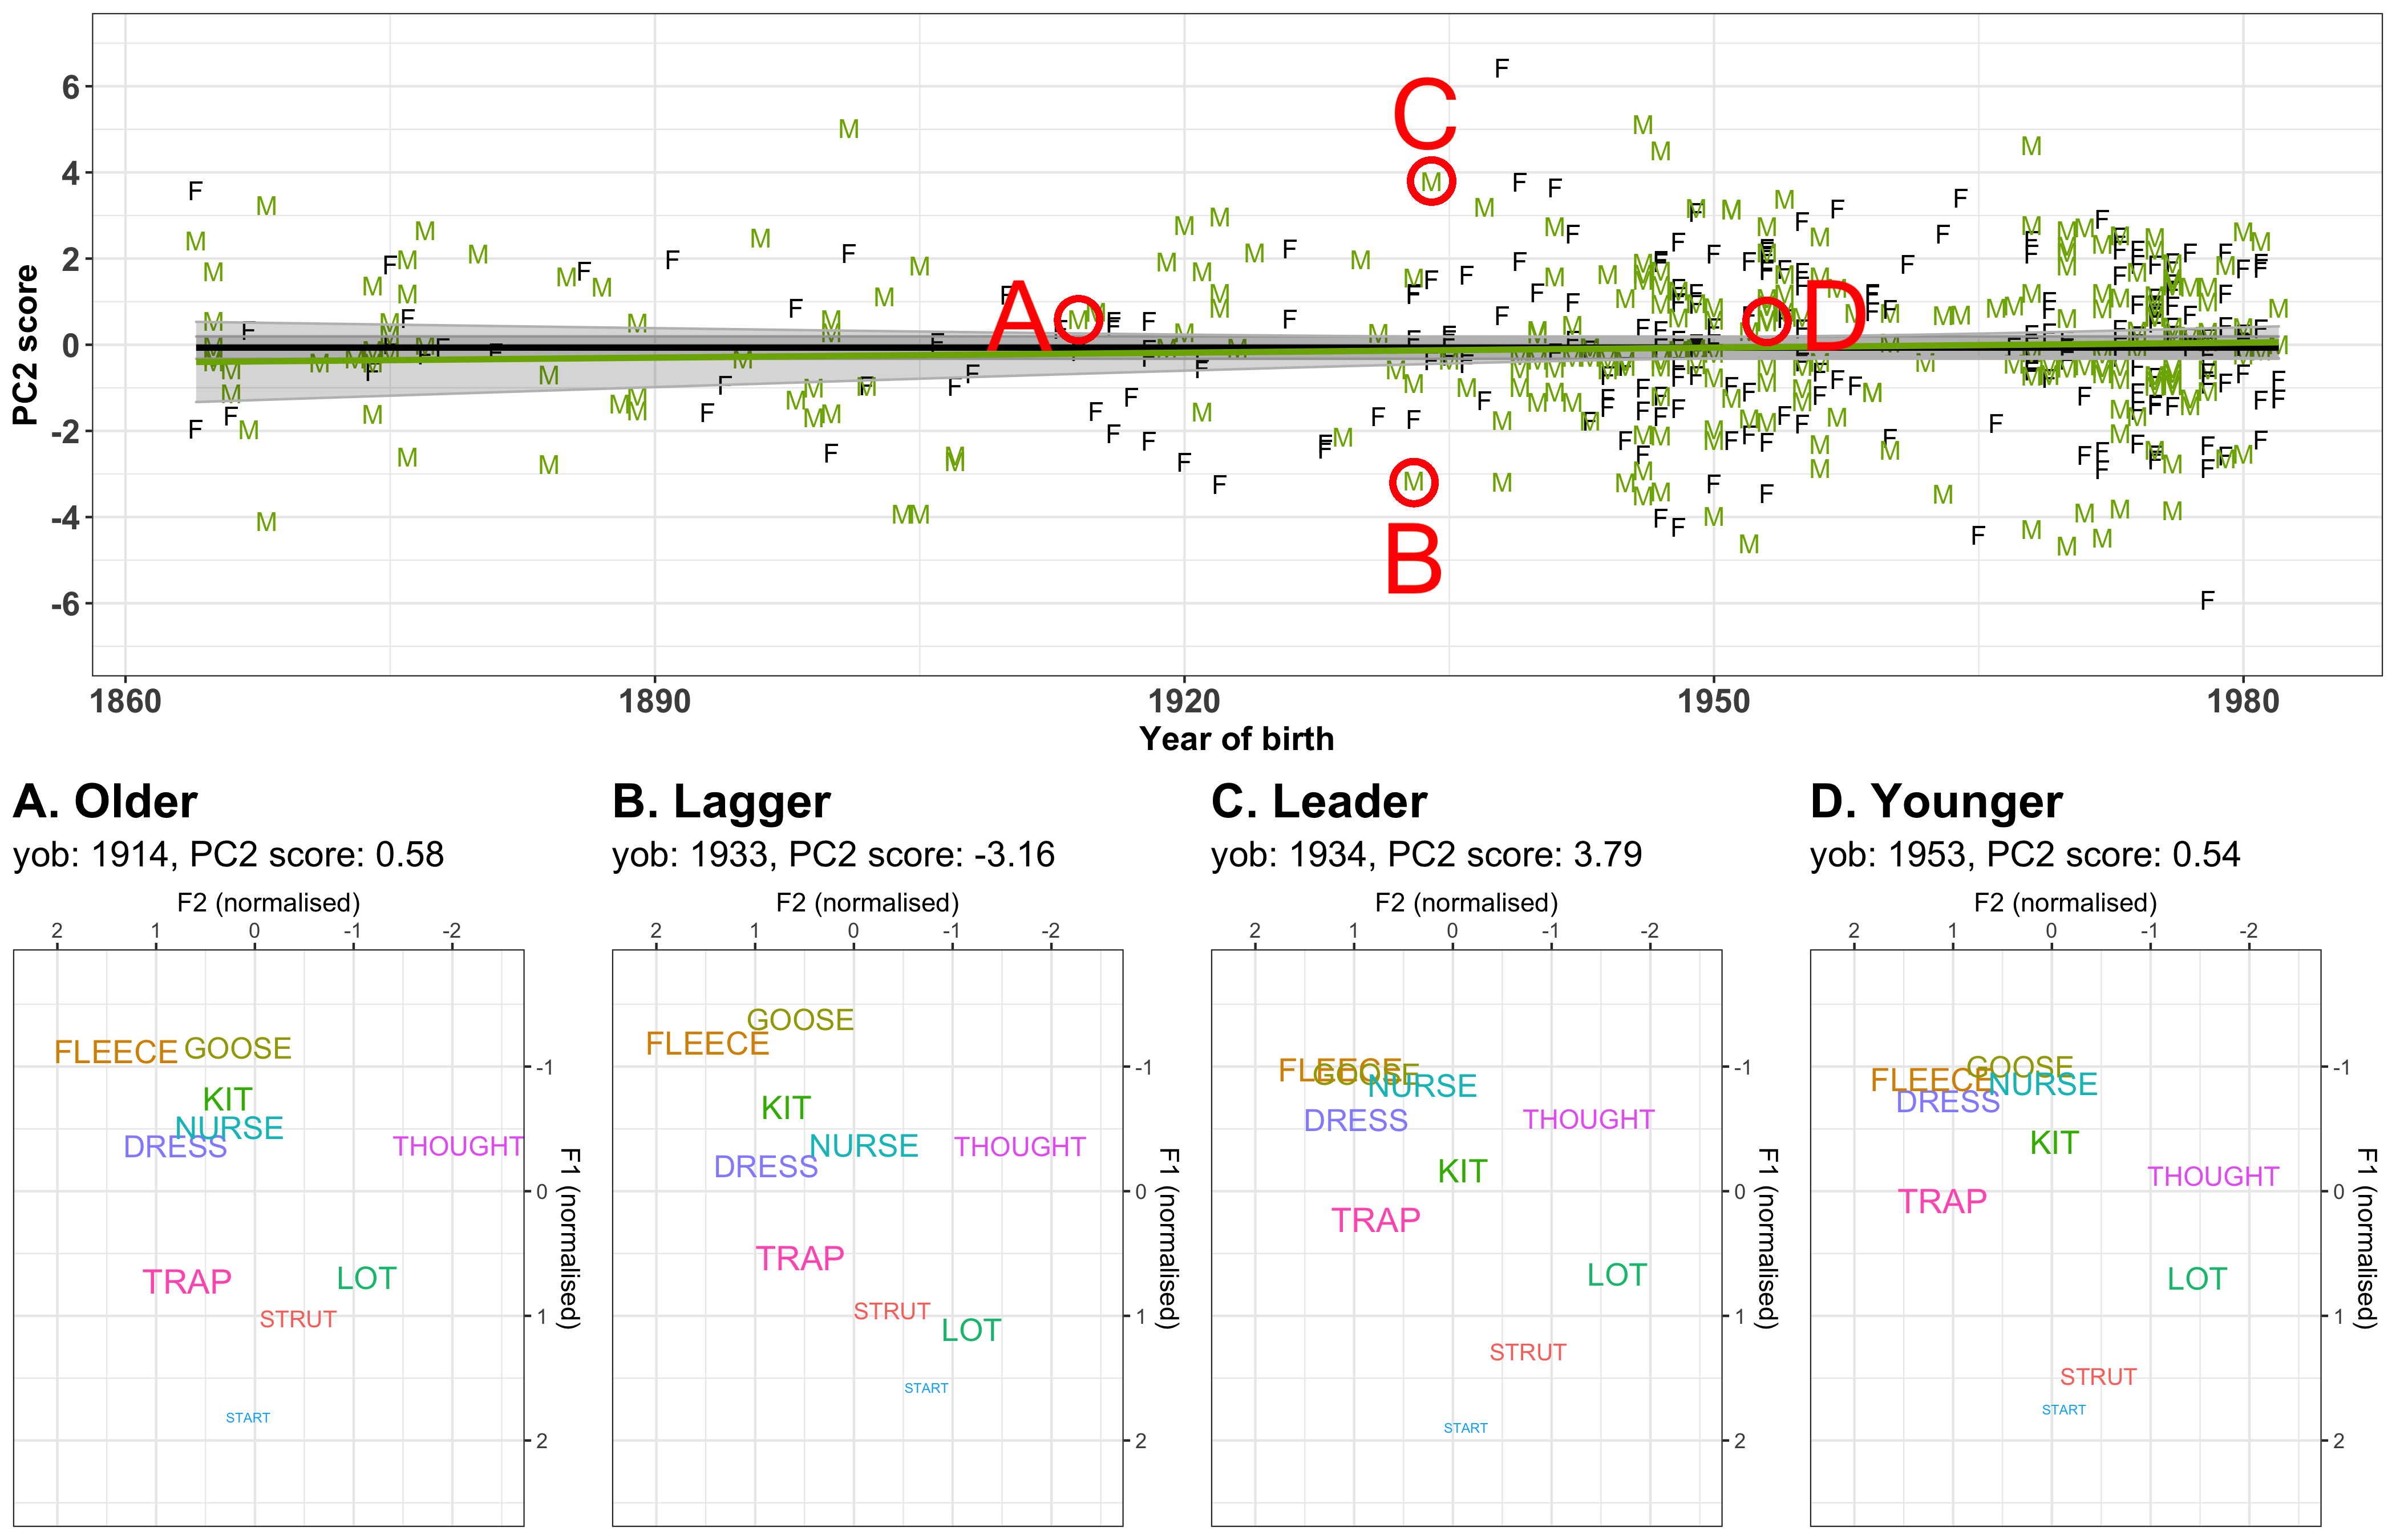
\includegraphics[width=\textwidth]{Figures/PC2_speaker_loadings_example.png}
\caption{\textbf{Top panel} Relationship between year of birth and speaker scores for PC2. Each black F and green M (for female and male speakers respectively) indicates an individual speaker in the data set. Two GAM smooths are fitted (green and black lines), highlighting the lack of relationship between year of birth and PC2 score for both genders. \textbf{Bottom panel} Two speakers with similar years of birth and gender have been circled to represent a negative and a positive score, with their vowel spaces given in \textbf{B} and \textbf{C} respectively.  Two speakers born 40 years apart have also been circled, who represent an older and younger speaker with PC2 scores close to zero for comparison, with their vowel spaces given in \textbf{A} and \textbf{D} respectively.}
\label{fig:PC2_speaker_loadings}
\end{figure}

\subsubsection{PC3: Adjacent vowel interactions at the front and the back}
\label{sec:PC3}

%%%%%%%
%PC3_variable_loadings
%%%%%%%

% \begin{figure}[!ht]
% \includegraphics[width=\textwidth]{Figures/PC3_plot_variables_combined.png}
% \caption{\textbf{A} Dot plot of the contributions of each vowel formant from PC3, the larger the contribution the more important that vowel formant is to the PC. vowel formants that are to the right of the red dashed line collectively contribute over 50\% to the PC. The +/- signs indicate the direction of the loadings. \textbf{B} Visualisation of how the loadings can be interpreted in terms of F1$\sim$F2 space. The location of the vowel label indicates the position of realisations made by speakers with low scores on PC3, with the trajectory ending at the position where speakers with highest scores are (based on GAMM smoothing). The size of the vowel label is indicative of the importance of the vowel to PC3.}
% \label{fig:PC3_variable_loadings}
% \end{figure}

%%%%%%%

The third PC accounted for 10.1\% of the total variance. Figure \ref{fig:PC3_variable_loadings}A gives the contributions for each of the vowel formants, in addition to a visualisation of how the PC can be interpreted in terms of the F1$\sim$F2 space (Figure \ref{fig:PC3_variable_loadings}B). There are four variables which appear to carry this co-variation: \textsc{lot} and \textsc{start} F1 and - to a slightly lesser degree - \textsc{dress} and \textsc{goose} F2.

%Inspecting Figure \ref{fig:sound_change} and/or the sound change animation, we are reminded that \textsc{lot} lowers and then raises, whereas \textsc{start} consistently lowers.  In terms of \textsc{dress} and \textsc{goose} F2, \textsc{goose} fronts dramatically and \textsc{dress} fronts slightly.  The fronting of \textsc{goose} is most vigorous amongst the earlier born speakers, whereas the fronting of \textsc{dress} is more vigorous in the later born speakers.

\begin{figure}[!p]
\includegraphics[width=\textwidth]{Figures/PC3_plot.png}
\caption{\textbf{A} Dot plot of the contributions of each vowel formant from PC3, the larger the contribution the more variance explained and therefore the more important that vowel formant is to the PC. vowel formants that are to the right of the red dashed line collectively contribute over 50\% to the PC. The $+/-$ signs indicate the direction of the loadings. \textbf{B} Visualisation of how the loadings can be interpreted in terms of F1$\sim$F2 space. The location of the vowel label indicates the position of realisations made by speakers with the lowest PC3 scores, with the trajectory ending at the position where speakers with the highest scores are. The size and colour of the vowel label is indicative of the importance of the vowel to PC3. \textbf{C} The trajectories of change for each vowel formant by year of birth (red line), with the speaker intercepts plotted as points around the trajectory. The colour of the points indicates the speaker's PC score, where green points are positive scores and black are negative. The contribution percentages for each vowel formant are given at the top of the panels and the most important vowel formants are highlighted by yellow boxes and the most important vowel formants are highlighted by yellow boxes.}
\label{fig:PC3_variable_loadings}
\end{figure}

If we look at the pairwise correlations (shown numerically in the \hyperref[sec:supplementarymaterials]{Supplementary Materials}), the strongest correlation amongst these vowels is a negative correlation between \textsc{start} F1 and \textsc{lot} F1 ($r = -.49$), whilst there is also a relatively strong correlation between \textsc{goose} F2 and \textsc{dress} F2 ($r = -.37$).  That is, this PC is driven by two particularly strong relationships: one at the front of the vowel space and one at the back.

The relationship with sound change can be seen in Figure \ref{fig:PC3_variable_loadings}C, in which we see how speakers with high/low PC3 scores are positioned in relation to the sound change trajectories. From this we see that speakers with high PC3 scores tend to have more innovative \textsc{start} F1.  \textsc{lot} F1 doesn't move in a consistent direction; thus speakers with high PC3 scores would vary in terms of innovativeness/conservativeness depending on their year of birth - earliest born speakers are conservative, but later born speakers are innovative. Whilst there is very little change in \textsc{lot} F1 over time, there is considerably more variation in the PC scores, suggesting that -- if this is linked to sound change -- the link is more likely to be via changes in \textsc{start} than \textsc{lot}, as \textsc{start} lowers in a linear direction over time.  Speakers with higher PC3 scores have an overall more innovative configuration, with these two vowels being more separated - a lower \textsc{start} and a higher \textsc{lot}.

A reasonable interpretation is that, in the back vowel space, PC3 captures the linear reorganisation of the space -- speakers with low PC3 scores have  \textsc{lot} and \textsc{start} close together, speakers with high PC3 scores have them far apart. This interpretation is reinforced by the inspection of slightly lower contributors to PC3 - we see that  \textsc{thought} and  \textsc{lot} are loaded in the same direction (Figure \ref{fig:PC3_variable_loadings}A). Speakers with high PC3 scores are overall more innovative with the back vowels. Recall that in PC1, we saw a repulsive force between \textsc{thought} F1/F2 and \textsc{start/strut} F2, with individual speakers either having \textsc{thought} raised and backed, or \textsc{start/strut} backed.  In PC3, by contrast we see speakers with high PC3 scores being more advanced in the separation between \textsc{lot/thought} F1 and \textsc{start} F1.  As \textsc{lot} (and to a lesser degree \textsc{thought}) raise, \textsc{start} lowers.  PC3 separates speakers who are more \textit{versus} less advanced in this process.

% Also loaded on PC3 are \textsc{goose} and \textsc{dress} F2. \textsc{goose} fronts over the time period.  High PC3 speakers are conservative for \textsc{goose}. \textsc{nurse} also fronts a lot over the time period and \textsc{nurse}, which has a weaker loading on PC3, in the same direction as \textsc{goose}.  So high PC3 speakers are conservative in the fronting of these vowels.

Moving to the front vowels, we see that \textsc{goose} and \textsc{dress} F2 also contribute to the PC. Speakers with high PC3 scores have a backer \textsc{goose}, indicating that they are conservative in relation to the direction of sound change. This trend is also seen in \textsc{nurse}, which although it contributes slightly less than \textsc{goose}, also fronts over time, but speakers with high PC3 scores produce more backed variants. In contrast to this, we see that those same speakers with high PC3 scores have fronter \textsc{dress}. Over time \textsc{dress} F2 is fairly stable for earlier born speakers, and then fronts.  Construed in terms of sound change, speakers with high PC3 scores are more innovative in the fronting of \textsc{dress}.  However, the change in \textsc{dress} over time is a much smaller effect than the change captured by the PC scores (i.e.\ there is much more variation in terms of the scores than there is from changes predicted by year of birth), suggesting that there may be some co-variation occurring here that is not solely due to the fact that \textsc{dress} is undergoing change.  Indeed, looking further down the vowel formant contributions, we see \textsc{trap} loaded in the same direction, and it shows even less movement than \textsc{dress} in F2 over time, but similar variation captured by PC3, with speakers who have high PC3 scores having fronter \textsc{trap}. Thus, the main patterns observed in the front vowels for this PC are that speakers with backer \textsc{goose/nurse} have fronter \textsc{dress/trap} and speakers with fronter \textsc{goose/nurse} have backer \textsc{dress/trap}.

 When we inspect individual vowel spaces, speakers with a high PC3 score uniformly have \textsc{dress} fronter than \textsc{goose}.  Many speakers with a low PC3 score actually have \textsc{goose} fronter than \textsc{dress} (see the Shiny app to explore these trends).  It appears that there is only room for one set of very front vowels.  If \textsc{dress} (and \textsc{trap}) are already occupying that space, there are limits to how far forward \textsc{goose} (and \textsc{nurse}) can move.  But for speakers with somewhat backer \textsc{dress/trap} (either because they are conservative in the mildly fronting sound change, or because their \textsc{dress/trap} vowels just happen to be a bit backer than the average population) there is an opportunity for \textsc{goose} and \textsc{nurse} to overtake them, and move to be the vowels at the very front edge of the vowel space.
 
Indeed, although the overall trajectories of \textsc{goose} and \textsc{nurse} show fronting, followed by very recent backing, consideration of the distribution around this trajectory (Figure \ref{fig:PC3_variable_loadings}C) shows that, even as these vowels back, a number of speakers maintain very front vowels.  Even when we have a trajectory of lowering of F2, there are still speakers who maintain a very high F2.  These are speakers with a low PC3.

\begin{figure}[!t]
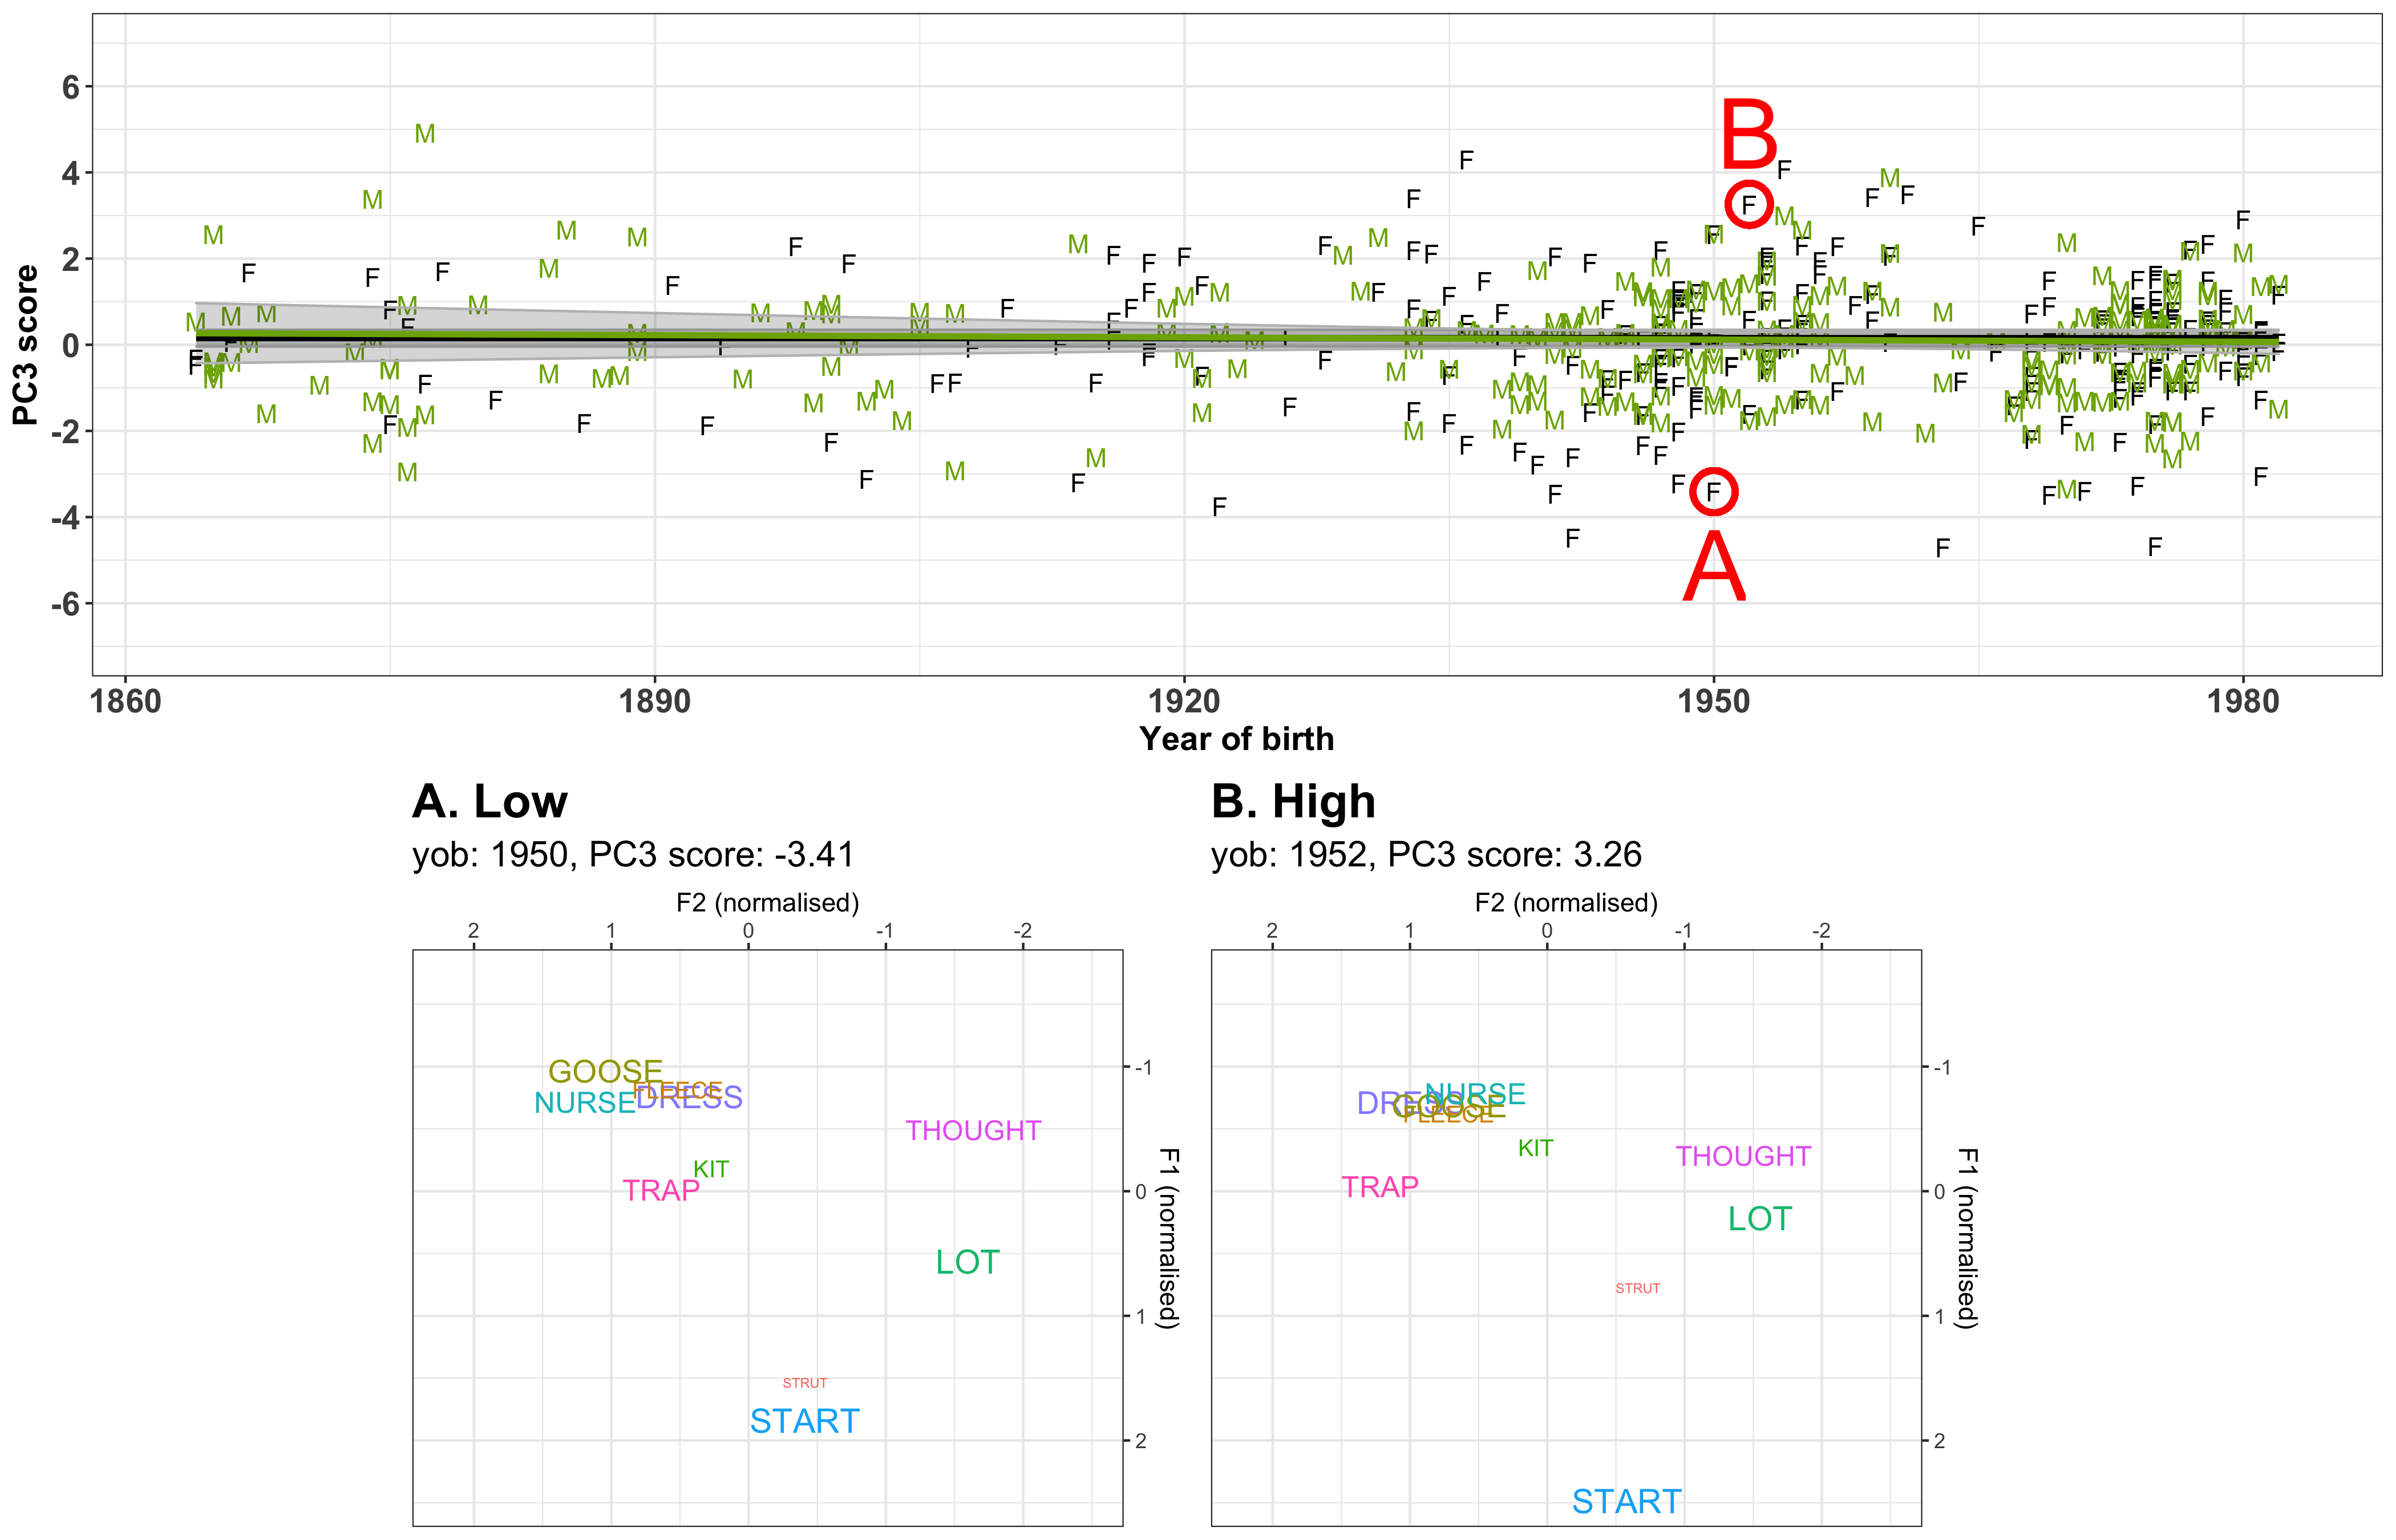
\includegraphics[width=\textwidth]{Figures/PC3_speaker_loadings_example.png}
\caption{\textbf{Top panel} Relationship between year of birth and speaker scores for PC3. Each black F and green M (for female and male speakers respectively) indicates an individual speaker in the data set. Two GAM smooths are fitted (green and black lines), highlighting the lack of relationship between year of birth and PC3 score for both genders. \textbf{Bottom panel} Two speakers with similar year of births and gender have been circled to represent a low and a high PC score, with their vowel spaces given in \textbf{A} and \textbf{B} respectively.}
\label{fig:PC3_speaker_loadings}
\end{figure}

Figure \ref{fig:PC3_speaker_loadings} shows two representative speakers with scores in opposite directions.  The speaker with a high PC3 score (speaker B) has \textsc{dress} (and \textsc{trap}) as the front-most mid-vowels and \textsc{goose} (and \textsc{nurse}) as more central.  For the speaker with a low PC3 score (speaker A), these vowels swap positions in terms of frontness - \textsc{goose} and \textsc{nurse} are the fronter vowels, and \textsc{dress} and \textsc{trap} are somewhat more centralised. At the same time, speaker A (with the fronted \textsc{goose}/\textsc{nurse} system) also has higher \textsc{start} and lower \textsc{lot} (i.e. they are more conservative in the position of \textsc{start}/\textsc{lot}).  This is also true -- to a lesser degree -- for \textsc{thought}. Speaker B, conversely has \textsc{start} and \textsc{lot} distinctly far apart in terms of F1.

In sum, PC3 tells us that, at any given time, those who are most advanced in the overall fronting of \textsc{goose} (and \textsc{nurse}), are those whose \textsc{dress} (and \textsc{trap}) vowels are slightly more central (and thus more conservative).  In other words, there is only space at the front of the vowel space for one pair of extreme front vowels. The speakers who are most advanced in the fronting of \textsc{goose} and \textsc{nurse} are most conservative in the elongation of the back vowels along the F1 space.

This may suggest that these two subsystems carry opposing social meaning, and/or that innovative speakers aren't necessarily `leaders' across the whole vowel space, but that different groups of speakers may concentrate their innovation in different subsystems of the vowel space.

% \begin{figure}[!ht]
% \includegraphics[width=\textwidth]{Figures/PC3_yob_important.png}
% \caption{GAMM smooths for vowel formants contributing to co-variation captured by PC3. Dotted lines show the trajectory of the formant over time -- from earlier born to later born speakers, for F1 (red) and F2 (blue) respectively.  Solid lines overlay the trajectory of the formant from speakers with low to high PC3 scores.}  
% \label{fig:PC3_yob}
% \end{figure}



%%%%%%%
%PC3_speaker_loadings
%%%%%%%

%%%%%%%

\subsection{Other pairwise correlations}

Finally, it is worth considering that the PCA is most suited to identifying patterns of co-variation that are carried by multiple co-varying vowels.  Any relationship between just two vowels, even if very strong, is unlikely to outrank a set of correlations carried across many vowels.  While most strong pairwise correlations are captured in the above analysis, one of the very strongest is not. There is a strong negative relationship between F2 \textsc{fleece} and F2 \textsc{nurse} ($r = -.58$).  Speakers with backer \textsc{fleece} have fronter \textsc{nurse}, and vice-versa.  This relationship does not appear above the 50\% threshold that we have used for interpreting any of the PCs, but both vowel's F2s feature somewhat below the 50\% threshold loaded in opposite directions in all three PCs.  This is a strong negative correlation, and our interpretation is the same as the negative relationship we saw between \textsc{dress} and \textsc{nurse} F2 in PC3.  There is only space for one set of very front vowels.  In each of Figures \ref{fig:PC1_speaker_loadings} and \ref{fig:PC3_speaker_loadings} for example, we see two vowel spaces, one with \textsc{nurse} the fronter vowel and one with \textsc{fleece} the fronter vowel.

\section{Discussion}

\subsection{Methodological Contribution}
Our primary goal was to develop a methodology that can be used to study co-variation, in order to start to address some of the major questions and predictions regarding co-variation in sociolinguistics and phonology. Our methodology successfully overcomes past limitations, and makes possible a system-wide analysis of co-variation.  

All sounds have changed over the time period we are studying (albeit some in a non-linear way).  Exploration of the supplementary Shiny app will quickly reveal that the vowel spaces of earlier born speakers are different from those of later born speakers.  Because the vowels are changing over this time period, therefore, they are all inherently correlated across speakers.  However, our model fitting procedure attempts to control for this type of year-of-birth-mediated co-variation, and this control appears to have been successful. In Figures \ref{fig:PC1_speaker_loadings}, \ref{fig:PC2_speaker_loadings} and \ref{fig:PC3_speaker_loadings} we see that the PCs we analyse capture co-variation between vowels, but crucially, this co-variation is independent of year of birth (and indeed gender). We have therefore found that there is correlational structure across speakers' vowel productions that is not simply due to the fact that the vowels are all simultaneously undergoing change.  This methodology, then, considerably broadens the data-sets that can be used to study patterns of co-variation: we are no longer limited to homogeneous data-sets of speakers of the same age and social background \citep{tamminga2019interspeaker}, as long as these factors can be controlled for by a mixed-effects modelling approach.

\subsection{New Zealand English: Summary of patterns of co-variation}
Our PCA has revealed three distinct clusters of co-varying vowels in NZE. It is important to note that these do not exhaust the sets of inter-relationships in the vowel space.  In particular, if there are two vowels that are very tightly linked, but work independently of all other vowels, this relationship is unlikely to have surfaced in the top 3 components.  

PC1 is related to a rearrangement of the back vowels, showing that individual speakers may have been innovative either in F1 for \textsc{thought} or in F2 for \textsc{strut/start/thought}, but they are unlikely to have been innovative in both at the same time. PC2 captures a set of vigorous vowel changes in NZE, including the NZE short front vowel shift.  Speakers who lead in one of these changes are likely to be leading in all of them.  The front vowels predominate in this cluster of vowel changes, but it is not exclusive to them -- the back vowel \textsc{lot}, for example, is also involved. PC3 distinguishes between leaders in the elongation of the back vowel space, and in the fronting of \textsc{goose} (and to a lesser extent, \textsc{nurse} in the front vowel space).  For these vowels, speakers are either innovative at the back, or the front, but not both.  The degree of \textsc{goose} fronting is also mediated by the frontness of \textsc{dress}. For speakers with a backer \textsc{dress} vowel, \textsc{goose} is able to move further forward, taking up a position as one of the frontest vowels in the vowel space. Such a relationship, between a vigorously fronting vowel, and an already front vowel, is also seen in the strong pairwise correlation between \textsc{nurse} and \textsc{fleece}.  \textsc{nurse} fronts and \textsc{fleece} backs -- speakers with backer \textsc{fleece} have fronter \textsc{nurse} and vice versa.

For ease of reference, the vowels linked together by the different PCs are illustrated in Figure \ref{fig:summary}. From this visualisation, it is easy to see that all vowels are included in at least one of the PCs, illustrating that there is no vowel whose production is independent of all the others.
There is clear evidence, then, that the vowels are not independent of each other, and that studying change in one vowel, independently of all others, requires understanding its relationship to other vowels, within the landscape of a full phonological vowel system.  This highlights the importance of a move toward studies of co-variation, and away from studies of the variation of specific vowels in isolation.

\begin{figure}[!t]
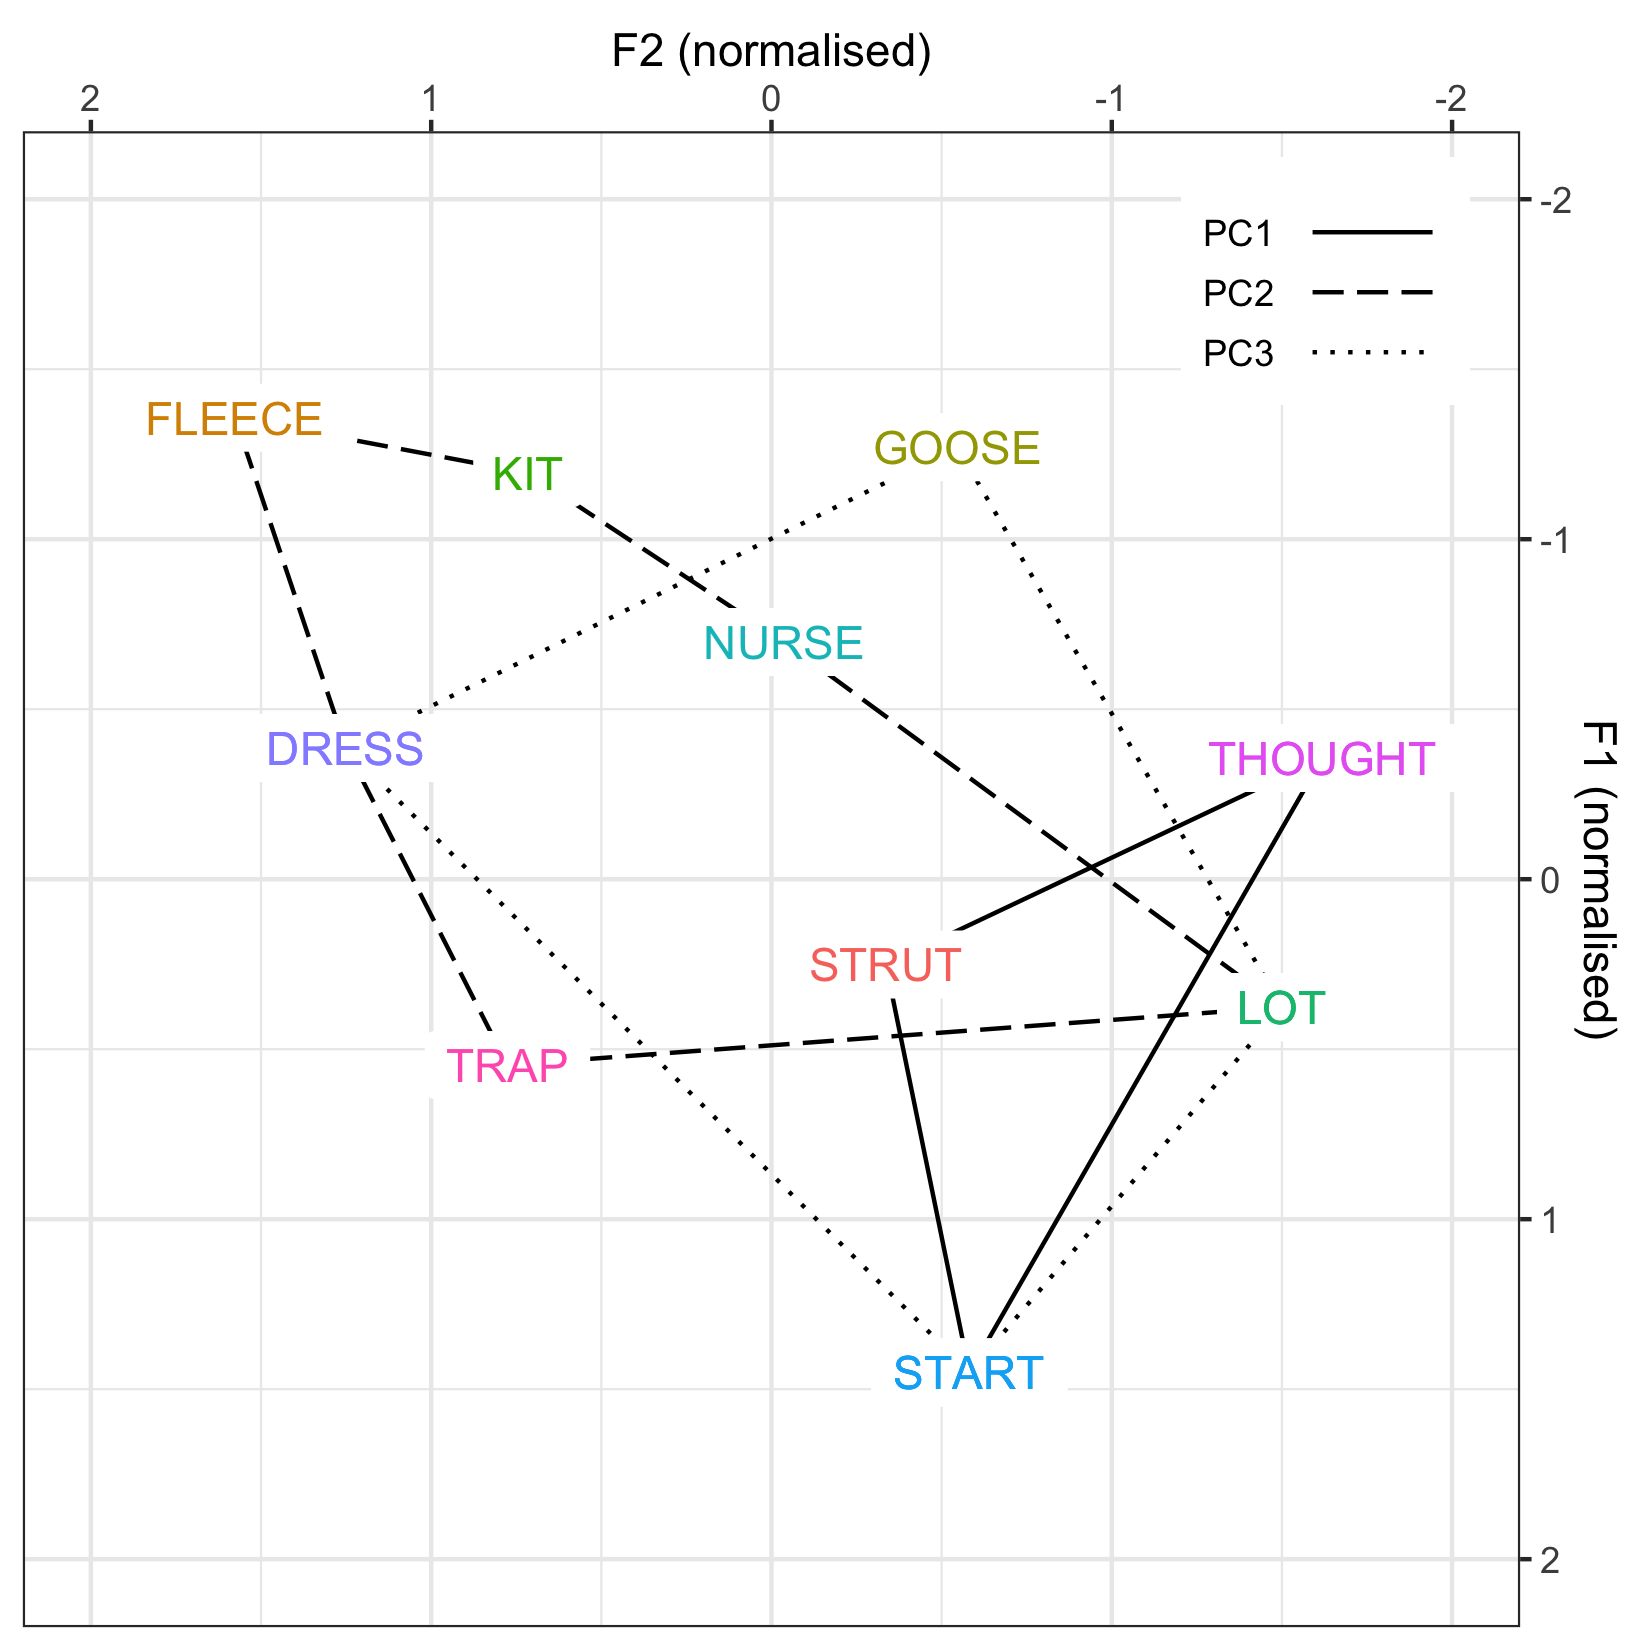
\includegraphics[width=\textwidth]{Figures/summary_PC.png}
\caption{Simple schematic showing vowel space (from an older speaker), illustrating the vowels linked together by PC1, PC2 and PC3}  
\label{fig:summary}
\end{figure}


\subsection{Research Question 1: Leaders and Laggers}

The first specific research question we had about NZE was about leaders and laggers of sound change.  We hoped to use this methodology and the NZE data-set to address
 \cite{guy2016linguistic}'s question about whether innovative variants tend to be used together by leaders or if different sets of changes are led by different speakers - our Research Question 1.

%``Are there socially identifiable leaders of change who tend to use all the innovative variants together, or are different innovations subject to differentiated social interpretations and individuated patterns of usage?'' .   

%Our data provide a mitigated `yes' answer to this question. 

The loadings on PC2 provide evidence that there are identifiable leaders/laggers for a sub-set of vowels.  This, however, does not imply that \textit{all} vowels need be involved. Over 50\% of the co-variation captured by PC2 involves movements in just 6 co-varying vowels.  While there are more that appear likely implicated, below the 50\% threshold, there are also others that are not loaded onto PC2 at all. 

Indeed, the full set of results provides clear evidence that if a speaker is a leader in one set of vowel changes, this does not imply they are a leader in all others.  In both PC1 and PC3 we see evidence that there are sets of vowels, such that if speakers are conservative for one, they tend to be innovative for another (e.g.\ PC3 -- lowering of \textsc{start} but fronting for \textsc{goose}).  This may mean that speakers concentrate their innovation in certain parts of the vowel space, or it may mean that there are different types of `leaders', in that different sound changes also carry different social meanings.  The proposal that several variables can cluster together because the speakers using them share social motivations or personas is consistent with the conclusions of smaller correlational studies examining this question \citep{becker2016linking, tamminga2019interspeaker}.

Our results demonstrate that there can indeed be leaders who use innovative variants for a substantial sub-set of phonetic variables (as shown by PC2). However, they also provide insights into how a speaker may exhibit opposing patterns, whereby the use of an innovative variant for one (or a number of) vowel(s) implies the use of a conservative variant for another (as shown by PC1 and PC3).  Previous literature investigating pairwise correlations between limited sets of phonological variables has reported positive correlations, but not, to our knowledge, negative ones. This again highlights the broad utility of our methodology to uncover such patterns of co-variation, whether they function in an aligned or indeed, an opposing manner.

\subsection{Research Question 2:  Are identified patterns of co-variation explainable by structural factors, or not?}


In addressing Research Question 2, it is first useful to note that none of the three PCs look like they are related to different overall articulatory biases, or normalisation failures. There is no pattern of strong cross-vowel co-variation in a particular direction that is limited to a particular part of the vowel space, for example, and we see no evidence of co-variation reflecting underlyingly different vowel space sizes. This suggests that the normalisation procedure we used achieved its goal.

There is also absolutely no evidence within this data of co-variation that can be linked to the phonetic implementation of a single feature (such as `high' or `back').  The sound change data does not show any such coordinated movement over time, and the PCs also do not reveal any patterns of this kind.  It is always possible that this co-variation may have existed, and could have been removed through the normalisation process, which scales the edges of the vowel spaces to cover the same area.  But the socially-driven parallel changes are certainly not explainable as artifacts of phonologically-driven parallel changes.

We do, however, see at least one pair of adjacent vowels which appear to move quite closely together. For earlier born speakers, \textsc{start} fronts while \textsc{strut} lowers.  Around 1920, \textsc{strut} is quite close to \textsc{start} and following this, they appear to undergo backing together (see Figure \ref{fig:PC1_variable_loadings}).  The F2 of both vowels is linked together on PC1, and there is a direct pairwise correlation of $r = .48$ -- the strongest positive pairwise correlation between vowels.  This is consistent with the interpretation that the primary difference between the two vowels in contemporary NZE is a quantity difference (and associated peripherality effects; see \citealt{warren2006oops, bauer2008new, warren2018quality}).

Some other adjacent pairs with reasonably high pairwise positive correlations are \textsc{lot} and \textsc{thought} F1 ($r = .34$) and \textsc{trap} and \textsc{dress} F1 ($r = .30$).  Unlike \textsc{start} and \textsc{strut} F2, these could also be explained by a chain-shifting relationship (as one is moving in the direction of the other) and we can also not eliminate the explanation that all three pairs are simply linked through social factors.  Thus, while there is no evidence that phonetic implementation of wholesale phonological features is responsible for our observed patterns, we do see some co-variation that is consistent with (but not conclusive of), parallel forces acting on some pairs of adjacent vowels.

With respect to known chain-shifts, there is a previously documented chain-shift involving (at least) \textsc{trap}, \textsc{dress} and \textsc{kit} \citep{hay2015tracking}, and these are all captured by PC2, which is aligned with these ongoing changes.  This could potentially be taken as evidence that the chain-shift exists within individuals -- if a speaker is a bit advanced in the raising of \textsc{trap}, for example, this pushes on their \textsc{dress}, and so on, leading them to be more advanced in the entire chain-shift. In this case, the chain-shifting mechanism could be construed to exist within individuals, and not just at a societal level.  However, a number of vowels are loaded onto PC2, and there is no strong evidence that the chain-shifting vowels are more closely interlinked than the other vowels in this PC (\textsc{lot} and \textsc{nurse}).  It is therefore not possible to tell whether chain-shifting has a causal effect on these vowels that is separate from the general finding that groups of speakers are leaders/laggers in this larger subsystem of vowels.

PC1 involves the expansion of vowels at the back into a linear organisation, with \textsc{strut} and \textsc{start} lowering and (eventually) backing, and \textsc{thought} raising and (eventually) fronting.  From PC1, we see that individuals were advanced either in the backing of \textsc{strut} or in the raising or \textsc{thought}, but not both.  This is consistent with the interpretation that these vowels are repelled from one another in a pushing relationship.  For some speakers, \textsc{thought} moves the quickest, removing the pressure on \textsc{strut}.   For some other speakers the backing of \textsc{strut} is more vigorous, and \textsc{thought} is slower to move. However, the PC suggests that there are few speakers who do not maintain the distance between these two sets of vowels through moving one or the other, which is consistent with a potential chain-shifting interpretation.  We note, too, that these vowels shift toward each other in duration over the timecourse of the corpus, with \textsc{strut} slightly lengthening, and \textsc{thought} considerably shortening\footnote{Many thanks to our anonymous reviewer for asking us to check this}. This reduction of the phonetic length distinction may well contribute to the repelling relationship in formant space. The full dynamics of this relationship are a prime target for future work. In particular, we might expect more detailed work to find differential effects of voiceless/voiced codas, as coda voicing has ramifications for the strength of the durational cue - as seen in interaction between \textsc{dress} and \textsc{fleece} in NZE \citep{maclagan2007getting}.

While PC1 contains vowels that are proximally close,  PC3, on the other hand, contains some vowels with opposite loadings that are more distant from each other, indicating that the existence of multiple social forces is also a distinct possibility.  The fact that we observe patterns of co-variation that are not obviously structurally linked  reinforces the prediction that follows from the sociolinguistic literature - that we should observe patterns of co-variation due to shared social meaning.  Patterns of co-variation with no apparent structural association are clear candidates for sites of socially-driven co-variation, although to prove this social link would require close sociolinguistic analysis, beyond the scope of this paper.

The question of the stylistic meaning of variants is intertwined with the question of leaders and laggers. In our data, all of the vowels are undergoing some change, so it is not possible to disentangle co-varying vowels that are changing from stylistic co-variation that is unrelated to change.  Certainly, the data generally supports the prediction from Eckert's work that there should be broad patterns of correlations across sets of variables, and that variables do not work in isolation of one another.  To definitively link this to different styles and speaker personas, we would need close and detailed stylistic analysis of the co-varying vowels in context.   In work in progress, we are analysing how vowels co-vary within individual speakers over the course of the conversation, which will enable us to more closely investigate how patterns of co-variation relate to patterns of social meaning - especially if the same sub-systems vary within individual speakers as observed across speakers \citep{brandvowelspace}.   Similar work on other languages and dialects may also help to identify which types of associations   tend to be observed across different contexts, suggesting some functional or linguistic pressure, and which are particular to specific contexts and are thus more suggestive of social factors.


Our analysis also assumes a constant degree of co-variation across the time period studied.  This may not be sufficient to account for vowels like \textsc{strut/start} which appear visually linked only in the later half of the data, and \textsc{lot/thought}, which both change direction during the time period studied.  If nascent structural co-variation becomes amplified by emergent social co-variation, this predicts increasing degrees of co-variation over a long time period. Further, if co-variation reflects leaders of particular sound changes, then such co-variation should be strongest during periods where the sound changes are most vigorous. Future analysis revealing how patterns of co-variation evolve and change over time will lead us still further toward understanding the mechanisms underlying patterns of co-evolution in the system as a whole.  Such nuances present clear methodological challenges beyond those tackled in this paper, and remain for future work.   A further over-simplification of the current analysis is the concentration on just two cues per vowel -- F1 and F2 extracted from the midpoint.  Other cues will also be relevant to a full study of co-variation, including durational cues, which are changing over time concurrently with the vowel formants, formant trajectories, and higher formants. These all influence the degree to which proximate vowels are confusable with each other, and thus the degree to which changes in those vowels might be interlinked. 



%\subsubsection*{Evolutionary pressures on the vowel space}

%Finally, it is not out of the question that some of the co-varying patterns result from overall evolutionary pressure.  Indeed chain-shifting itself arises from a pressure that maximises dispersion and contrast \citep{labov1994principles, gordon2002investigating, hay2015tracking}.  The interlinked vowels at the back, which move to a linear organisation, are likely influenced by such forces, and are related to each other both through PC1 and PC3.

\subsection{Overall Summary}

Our methodology presents a way of controlling for known overarching influences on production patterns, and identifying subsystems of vowel productions -- vowels whose productions are not independent of each other. Using these methods, we find that all vowels work together as part of a complex system. There is no vowel which is not strongly loaded onto at least one of the three PCs we discuss.  That there are three separate components shows that there is some structure to the co-variation -- each vowel is more tightly linked to some subset of vowels than to others.

The most compelling evidence from our results addresses the question of whether there are overall `leaders' and `laggers' in sound change.  Our analysis provides evidence that sound changes that are not independent of each other are also not necessarily linked structurally.  For some vowels, if we know that a speaker is advanced in that vowel change, it follows that they are also likely to lead in a constellation of other, possibly unrelated, vowel changes.   It is not the case, however, that a speaker's being a leader in one vowel change implies that they are a leader in all vowel changes.  

In terms of identifying whether linkages are structural or social, there is only so far we can go with the current data-set and analysis.   We identified some local patterns of co-variation which may be related to chain-shifting, repulsive relationships, or close linkages of proximate vowels.  However, there are other patterns of co-variation where there is no clear structural relationship.  A likely explanation for such co-variation is that the vowels are linked through shared social meaning. Indeed, we cannot yet eliminate this explanation for any of the patterns of co-variation observed. That is -- just because there is a plausible structural link between vowels, it does not follow that the observed linkage is indeed solely structural. To fully confirm whether any of the observed patterns of co-variation are related to underlying social meaning, we would need, at the very least, close stylistic analyses that reveal the social meanings when the variables are observed in usage. Indeed, it seems unlikely that linked social meanings between vowels arise entirely accidentally.  While not all the observed co-variation can be explained by them, there are many hints of structural relationships in our data.  If independent reasons exist for vowels to be linked -- whether through chain-shifting (\textsc{trap/dress/kit}), a mutual pushing relationship (\textsc{strut/thought}), closely parallel productions (\textsc{strut/start}), or jostling for the edge of the vowel space (\textsc{goose/dress}) -- and this leads them to co-vary within the same speakers, this likely provides the seeds for similar social meanings to become associated with correlated variants of the vowels.  Most or all of the proposed mechanisms underlying co-variation patterns may exist, and conspire to create strong patterns of co-variation: sub-systems of co-varying vowels.

Finally, studying the NZE monophthongs as a system has revealed several interesting relationships and sound changes within the time-course of our data set that have not previously received much attention.  First, while much previous research has focused on the short front vowels, we present here new insights into how there has also been a considerable rearrangement of the back vowels.  The rearrangement of this system has perhaps been less apparent in research because the vowels have tended to be analysed independently of each other. What we do observe is that these vowels undergo a number of non-linear changes (most notably in \textsc{start} and \textsc{thought} F2), before arriving to their contemporary arrangement.
% as the movements of the vowels involved are not monotonic; the vowels show movement in the F1$\sim$F2 space before arriving in their contemporary linear arrangement.
The PCA results clearly reveal that these movements are interlinked.  Second, while the fronting of \textsc{goose} and \textsc{nurse} has been widely commented upon, the consequences of them potentially colliding with the front vowels (\textsc{fleece, dress, trap}) have not.  The sound change trajectories (cf.\ Figure \ref{fig:sound_change}), show that toward the end of the time period, \textsc{goose} and \textsc{nurse} start to back again, while \textsc{dress} fronts.  However, PC3 (and the pairwise correlation between \textsc{fleece} and \textsc{nurse}) reveals that for some speakers, the fronting vowels are able to `overtake' the previous frontest vowels, and become the frontest in the vowel space (see speakers with low PC3 in the Shiny app, and the examples in Figure \ref{fig:PC3_speaker_loadings}). The degree to which this is possible interacts with how front the speaker's \textsc{fleece, dress} and \textsc{trap} vowels are.  There is thus some jostling for the frontest part of the vowel space, which would not be apparent if each vowel's trajectory was analysed independently of all the others. 

\section{Conclusions}

There are many reasons to expect that vowels will operate together as a co-ordinated system. However, the study of such patterns of co-variation across individual speakers has previously been methodologically challenging.  We have presented a methodology enabling the systematic study of co-variation across different phonemes.  We present a novel approach that controls for known predictors of co-variation, and finds clusters of variables that are linked systematically. Applying this to a data-set of NZE which has considerable time-depth, we find strong evidence of patterns of co-variation, which leads us to the conclusion that no vowels in our data operate independently of each other.  

Some observed relationships are predicted from literature that has already proposed structural relationships (the NZ short front vowel shift). Whereas, there are other relationships that seem to suggest previously overlooked structural relationships, including a linear reorganisation of the back vowels, driven by a repulsive relationship between \textsc{thought} and \textsc{strut/start}; and jostling amongst the high front vowels for the frontest part of the vowel space.  

Not all observed relationships can be explained through such structural relationships, though, and indeed we see cases in which vowels may be linked together socially -- for example, in PC2, where we have innovative versions of many vowels clustering within speakers (`leaders' of these changes).  Such social co-variation between vowels does not always go in the same direction, as in both PC1 and PC3, where innovation in one set of vowels is linked with conservatism in the other.  Once we accept that a likely explanation for some co-variation is social, we are unable to rule out the possibility that all the co-variation we observe is of this kind.  However, it seems very likely that structural relationships play some role, perhaps seeding potential social interpretations, which then strengthen the emergent patterns of co-variation.

To fully disentangle the interpretations, some close sociolinguistic analysis of the speakers, discourse, and use of variants in context is needed, and this is a clear direction for future work.  This paper provides a methodology (and associated code - see supplementary materials) to allow systematic analysis of co-variation across languages and dialects, and paves the way for comprehensive analyses of factors that underpin co-variation across speakers. 

The study of how vowels change over time has traditionally examined individual vowels. When examining change in any particular vowel, research tends to find socially meaningful distributions of speakers, with speakers on the margins of the distribution representing `leaders' or `laggers' in that particular change. But it has proven challenging to move beyond individual variables, towards an understanding of sound systems.  We have provided a significant step forward in this endeavour, by overcoming long-standing methodological challenges to the understanding of co-variation.  Our analysis provides novel insights into the structure of sound systems, demonstrating the existence of structured patterns in individuals' realisations of specific vocalic variables across a large group of speakers.

\vfill
\newpage

\section*{Acknowledgements}
\noindent This research was made possible by a Royal Society of New Zealand Marsden Research Grant (17-UOC-049). The authors would like to thank members of the New Zealand Institute of Language, Brain and Behaviour for their feedback and comments as this work progressed. Earlier versions of this work were presented at the International Congress of Phonetic Sciences, Melbourne, Australia 2019 and LabPhon17, 2020 and benefited from feedback and discussions at both events. The current version has benefitted immensely from detailed comments from Jonathan Harrington, and two other anonymous reviewers.  The ONZE data was collected by the Mobile Disc recording Unit of the NZ Broadcasting Service, Rosemary Goodyear, Lesley Evans, members of the NZ English class of the Linguistics Department, University of Canterbury, and members of the ONZE team. The Canterbury Regional Survey was co-ordinated by Alex D'Arcy. The work done by members of the Origins of New Zealand English Project (ONZE) in preparing the data, making transcripts, and obtaining background information is also gratefully acknowledged. The Corpus was created and supported with funding from the following sources: University of Canterbury, Foundation for Research, Science and Technology (the New Zealand Public Good Science Fund), the Royal Society of New Zealand, The New Zealand Lotteries Board Fund, and the Canterbury History Foundation.    We are particularly grateful to Robert Fromont for his work programming LaBB-CAT – the ONZE Corpus search engine and interactive interface.

\section*{Supplementary Materials}
\label{sec:supplementarymaterials}

\noindent All files referred to in this manuscript as being in the Supplementary Materials can be accessed via:

\begin{itemize}
    \item The online GitHub repository at:\\ \url{https://github.com/nzilbb/Covariation_monophthongs_NZE}
    \item The Open Science Framework at:\\ \url{https://osf.io/q4j29/}
    \item The online Shiny app (including the animated vowel spaces) can be accessed at:\\
    \url{https://onze.shinyapps.io/Covariation_shiny/}
\end{itemize}

\noindent Both the GitHub and OSF repositories contain the same files (including the data, data filtering and analysis scripts and the Shiny application). The analysis file also contains additional analyses that were not considered crucial for inclusion in the paper, but may be of interest to readers. For readers not familiar with GitHub or OSF, you can access individual files at \url{https://nzilbb.github.io/Covariation_monophthongs_NZE/}. You will need to install R in order to run some of these files.

\vfill

\bibliography{References/Covariation_references.bib}

\end{document}